\documentclass[11pt]{amsart}

%Packages.

\usepackage[parfill]{parskip}
\usepackage{verbatim}
\usepackage{amsmath}
\usepackage{amssymb}
\usepackage{amsfonts}
\usepackage{amsthm}
\usepackage{mathrsfs}
\usepackage{tikz}
\usetikzlibrary{matrix,arrows}
\usepackage[all]{xy}
\usepackage{mathrsfs}
\usepackage{a4wide}
\usepackage{enumerate}
\usepackage{hyperref}
%\usepackage{showkeys}

%Theorem styles.

\theoremstyle{plain}
\newtheorem{conj}{Conjecture}
\newtheorem*{thm}{Theorem}
\newtheorem{theorem}{Theorem}%[section]
\newtheorem{lemma}[theorem]{Lemma}%[section]
\newtheorem{proposition}[theorem]{Proposition}%[section]
\newtheorem{corollary}[theorem]{Corollary}%[section]
\newtheorem{claim}[theorem]{Claim}%[section]
\newtheorem{question}[theorem]{Question}
\newtheorem{conjecture}[theorem]{Conjecture}


\theoremstyle{definition}%[section]
\newtheorem{definition}[theorem]{Definition}%[section]
\newtheorem{example}[theorem]{Example}%[section]
\newtheorem{project}{Project}

\theoremstyle{remark}%[section]
\newtheorem{remark}[theorem]{Remark}%[section]

%\numberwithin{theorem}{section}

\newcommand{\G}{\mathcal{G}}
\newcommand{\E}{\widehat{E}}
\newcommand{\X}{\widehat{X}}
\newcommand{\A}{\widehat{A}}

\newcommand{\ucong}{\rotatebox{90}{$\cong$}}

\title{Inverse semigroup theory and the K-theory of certain operator algebras.} 
\date{January 2013}
\author{Martin Finn-Sell}
\email{Martin Finn-Sell: ms1205@soton.ac.uk}

\begin{document}
\bibliographystyle{alpha}

\maketitle

\begin{abstract}
Inverse semigroup $C^{*}$-algebras arise in many interesting ways in $C^{*}$-algebra theory, particularly from graph and tiling algebras. A specific point of interest is their operator K-theory. In this paper a new connection is made to the K-theory of reduced group $C^{*}$-algebras, adapting techniques that arise first in work of Pimnser and Voiculescu concerning K-theory for free group $C^{*}$-algebras and then later in work of Brodzki, Niblo and Wright in a more general setting. We construct analogues of the well known Pimsner-Voiculescu short exact sequence in the context of certain inverse semigroups and the relate these techniques to a coarse geometric object known as a partial translation structure. We give examples of these ideas by considering specific partial translation stuctures and their groupoids.
\end{abstract}

\section{Introduction.}
The work of Pimsner and Voiculescu on operator K-theory was fundamental, particularly the development of K-theory exact sequences associated to actions of free groups on $C^{*}$-algebras via automorphisms \cite{MR670181,MR587369}. To motivate the importance of these results, consider the case of a free group $F_{n}$ acting by (trivial) automorphisms on a point. The sequence constructed gives a computation of the K-theory of the reduced group $C^{*}$-algebra $C^{*}_{r}(F_{n})$ \cite{MR670181}. 

The construction relies on the geometry of the group $F_{n}=\langle a_{1},...,a_{n} | \rangle$; consider $2n$-regular tree, which is the Cayley graph of $F_{n}$, and then consider the subset $X$ of this graph given by considering all words that do not begin with $a_{1}^{-1}$. The key idea is then to consider the truncation of the group operation to this subset, which then extends to a representation of the group on the Hilbert space $\ell^{2}(X)$ by partial isometries. Denote by $C^{*}\mathcal{T}_{n}$ the $C^{*}$-algebra generated by these partial isometries. This is algebra was shown to have the same K-theory as $C^{*}_{r}(F_{n-1})$ and is connected to $C^{*}_{r}(F_{n})$ by a natural short exact sequence, now called the \textit{Pimsner-Voiculescu short exact sequence}:
\begin{equation*}
0 \rightarrow \mathcal{K}(\ell^{2}(X)) \rightarrow C^{*}\mathcal{T}_{n} \rightarrow C^{*}_{r}(F_{n}) \rightarrow 0
\end{equation*}
These, together with careful analysis of the maps between K-theory groups, provide the inductive computation of $K_{*}(C^{*}_{r}(F_{n}))$. The method presented here of truncating to a subspace of the Cayley graph has since been extended by Lance \cite{MR723010} to deal with certain free products and Pimnser \cite{MR860685} to deal KK-theoretically with any group that acts freely on a tree. We remark that these ideas have been extensively developed and extended by Brodzki, Niblo and Wright \cite{BNW-KTA}.

We observe that the operator and geometic truncations outlined above are directly associated to the notion of \textit{enlargement} \cite{MR2221438} from inverse semigroup theory. In particular, restricting a group action on a suitable space to a subspace gives rise to \textit{Inverse monoids}, each of which satisfies many natural properties that should be associated to the original group action. The exploration of this connection between inverse semigroup theory and partial or restricted group actions is the main theme in this paper.

Inverse monoids play in important role in both geometry and topology, and have a rich and well studied connection to operator algebras; many natural examples from the subject can be described using inverse monoid algebras \cite{MR1798993,EGS-2011,mypub1}. In this paper we will focus specifically on the class of \textit{F-inverse monoids}. This class contains, and is a prototypical example of, the truncations of group actions on subspaces that are in some sense \textit{deep} in the group. To such inverse monoids we associate (in Theorem \ref{thm:PV1}) a short exact sequence that generalises the Pimsner-Voiculescu short exact sequence. Explicitly we prove:

\begin{thm}\label{thm:IT1}
Let $S$ be an F-inverse monoid and let $\G_{\E}$ be its universal groupoid and let $A=C_{c}(\G_{U})$. Then we have the following (intrinsic) short exact sequence of $C^{*}$-algebras:
\begin{equation*}
0 \rightarrow \overline{A} \rightarrow C^{*}_{r}(\mathcal{G}) \rightarrow C^{*}_{r}(G) \rightarrow 0
\end{equation*}
\end{thm}

This result is used in a later section to compute the K-theory of certain restrictions within free groups related to the work of Pimsner-Voiculescu and Lance \cite{MR670181,MR723010}. We show that this inverse semigroup sequence captures new behavour in this instance and we connect this to the work of \cite{BNW-KTA} using the concept of a partial translation structure \cite{MR2363428}.

Additionally, we give some results in the case that the inverse monoid $S$ has a zero element; the monoids for which we have results, called strongly 0-F-inverse monoids, are plentiful and easily constructed from groups.

\begin{thm}\label{thm:IT2}
Let $S$ be a strongly $0$-F-inverse monoid with universal group $G:=U(S)$. If $G$ is $K$-exact then the sequence:
\begin{equation*}
0 \rightarrow C^{*}_{r}(\G_{U}) \rightarrow C^{*}_{r}(\G_{\E}) \rightarrow C^{*}_{r}(\G_{\E_{tight}}) \rightarrow 0
\end{equation*}
is exact at the level of K-theory.  
\end{thm}

This case proves challenging to access directly as the structure of the reduced $C^{*}$-algebra is much more complex. The primary idea that provides an avenue to study these objects is a result of Milan and Steinberg \cite{Milan-Steinberg}, which describes the critera necessary to get Morita equivalences between the universal groupoid $\G_{\E}$ and some transformation groupoid built from the universal group associated to $S$. As an example, it is possible to construct the Cuntz extension using this technique. This construction is provided in Section \ref{sect:S2} and it is closely related to ideas in the work of Cuntz, Echerhoff and Li on K-theory of Semigroup $C^{*}$-algebras \cite{CEL-2}.

Lastly, a new proof of the nonexactness of Gromov monster groups \cite{MR1978492,exrangrps} is given. This relies heavily on all the ideas developed in the latter half of the paper.

The remainder of this section contains preliminary material, focusing on the combinatorial and geometric aspects of inverse semigroups and their related groupoids.

\subsection{The basics of inverse semigroup theory.}

A \textit{semigroup} is a set $S$, together with an associative binary operation. If additionally it has a unit element, then we say it is a \textit{monoid}.

\begin{definition}\label{Def:invsemi}
Let $S$ be a semigroup. We say $S$ is $inverse$ if there exists a unary operation $*:S \rightarrow S$ satisfying the following identities:
\begin{enumerate}
\item $(s^{*})^{*}=s$
\item $ss^{*}s=s$ and $s^{*}ss^{*}=s^{*}$ for all $s \in S$
\item $ef=fe$ for all idempotents $e,f \in S$ 
\end{enumerate}
\end{definition}

A very fundamental example of such an object is the \textit{symmetric inverse monoid} on any set $X$; consider the collection of all partial bijections of $X$ to itself, giving them them the natural composition law associated to functions - that is find the largest possible domain on which the composition makes sense, shown below in Figure \ref{Fig:Comp}.


\begin{figure}[h]
\begin{center}

%Def of Circles needed
\def\firstcircle{(-0.25,-1.25) circle (1.0cm)}
\def\secondcircle{(-0.25,0) circle (1.0cm)}
\def\thirdcircle{(-4.75,0) circle (1.0cm)}
\def\forthcircle{(-4.75,-2.5) circle (1.0cm)}
\def\fifthcircle{(-4.75,-1.25) circle (1.0cm)}

\tikzset{filled/.style={fill=circle area, draw=circle edge, thick},
    outline/.style={draw=circle edge, thick}}
    
\setlength{\parskip}{5mm}
% Set A and B
\begin{tikzpicture}
    \begin{scope}[fill opacity=0.5]
        \clip \firstcircle
              \fifthcircle;
        \fill[filled] \secondcircle
                      \thirdcircle
                      \forthcircle;
        \end{scope}
               
    %\draw[outline]    
    \draw[outline] \firstcircle node [below] {$dom(f_{2})$};
    \draw[outline] \secondcircle node [above] {$im(f_{1})$};
    \draw[outline] \thirdcircle node [above] {$dom(f_{1})$};
    \draw[outline] \forthcircle node [below] {$im(f_{1})$};
        %\node[anchor=south] at (current bounding box.north) {$A \cap B$};
    \draw[>=stealth,->,thick] (-3.25,0) -- node [above] {$f_{1}$} (-1.5,0);
    \draw[>=stealth,->,thick] (-1.5,-1.5) -- node [above] {$f_{2}$} (-3.5,-2.5);
    \draw (-6.75,-0.85) node {$dom(f_{2}\circ f_{1})$};
    \draw (-6.75,-1.75) node {$im(f_{2}\circ f_{1})$};    
    \draw[outline] (-8.5,-4) rectangle (2.25,1.5);
    \draw (1.75,-3.25) node {$X$};
\end{tikzpicture}

\caption{The multiplication of partial bijections}
\label{Fig:Comp}
\end{center}
\end{figure}
Explicitly:
\begin{equation*}
f_{2}\circ f_{1}: f_{1}^{-1}(im(f_{1})\cap dom(f_{2})) \rightarrow f_{2}(im(f_{1})\cap dom(f_{2})).
\end{equation*}

A key observation that makes connects the combinatorial aspects of inverse semigroup theory to the geometry of partial bijections is the following result of Wagner and Preston \cite{MR1455373}:

\begin{theorem}\label{Thm:WP}
Let $S$ be an inverse semigroup. Then there exists a set $X$ such that $S \hookrightarrow I(X)$.
\end{theorem}

When $X$ is a metric space we will be considering a inverse submonoid of $I(X)$ in which every partial bijection that maps elements only a finite distance, that is a generalised (or partial) translation. We denote this by $I_{b}(X)$.

\begin{definition}
Let $S$ be an inverse monoid. We denote by $E(S)$ the semilattice of idempotents (just by $E$ if the context is clear). This is a meet semilattice, where the meet is given by the product of $S$ restricted to $E$. In this situation, we can use the following partial order:
\begin{equation*}
e \leq f \Leftrightarrow ef=e
\end{equation*}
we make use of this order later.
\end{definition}

We remark that for a metric space $X$ every idempotent element in $I(X)$ moves elements no distance, and hence $E(I(X))=E(I_{b}(X))$. An inverse submonoid with this property is often called \textit{full}.

We want to consider quotient structures of an inverse monoid, and unlike in group theory where we have the concept of a \textit{normal} subgroup our subsemigroups will not in general possess enough information. One possible choice is to consider \textit{ideals} in $S$. 

\begin{definition}
Let $I$ be a subset of $S$. $I$ is an ideal of $S$ if $SI \cup IS \subset I$.
\end{definition}

From an ideal we can get a quotient - at the cost of a \textit{zero element}, that is an element such that $0s=s0=0$ for all $s \in S$.

\begin{definition}
Let $S$ be an inverse monoid and let $I$ be an ideal of $S$. Then we can define $\frac{S}{I}$ to be the set $(S \setminus I) \cup \lbrace 0 \rbrace$, equipped with the following product:
\begin{eqnarray*}
s \Xst t = \left\lbrace \begin{array}[c] $st$ \mbox{if} s \mbox{and} t \not\in I \\ 0 \mbox{ if } s \mbox{ or } t \in I \end{array}
\end{eqnarray*}
This is an inverse monoid with 0 called the \textit{Rees quotient} of $S$ by $I$.
\end{definition}

In general quotients are given by equivalence relations, and in order to get an inverse monoid from the equivalence classes it is enough to impose a closure on the relation. A relation of this type is called a \textit{congruence} on $S$.

\begin{definition}
An equivalence relation $\sim$ on $S$ is called a \textit{congruence} if for every $u,v,s,t \in S$ such that $s \sim t$, we know that $su\sim tu$ and $vs \sim vt$. This allows us to equip the quotient $\frac{S}{\sim}$ with a product, making it into an inverse monoid.
\end{definition}

We consider a specific congruence on $S$ called the minimum group congruence.  This congruence, denoted by $\sigma$, is given by:
\begin{equation*}
s \sigma t \Leftrightarrow (\exists e \in E) es = et
\end{equation*}
A congruence is \textit{idempotent pure} when $e \sim s$ if and only $s \in E$. This collects all idempotents into classes when we quotient out. The minimum group congruence, on the class of E-unitary inverse monoids, is an example of an idempotent pure congruence. Additionally it is the smallest group congruence on $S$ \cite{MR1694900}.
\begin{definition}
An inverse monoid $S$ is called E-unitary if for all $e \in E$ and $s \in S$ if $e \leq s$ then $s \in E$. $S$ is F-inverse if the preimage of each $g \in \frac{S}{\sigma}$ has a maximum element in the order on $S$. We denote these maximal elements by $Max(S)$, and we remark that this is equivalent to asking that for every element $s \in S$ there exists a \textit{unique} maximal element $t \in S$ such that $s \leq t$.
\end{definition}
For an F-inverse monoid it is possible to study the minimum group congruence by considering all the maximal elements with a new product:
\begin{equation*}
(\forall s,t \in Max(S)) s \Xst t = u \mbox{ for } !u \in Max(S) \mbox{ with } st \leq u.
\end{equation*}

In general the inverse monoids we are considering in this paper will not be as nice as this: they will have a zero element. However we can still make similar generalisations of the above definitions:

\begin{definition}
We say $S$ is 0-E-unitary if $\forall e \in E\setminus 0, s \in S$ $e \leq s$ implies $s \in E$. We say it is 0-F-inverse if there exists a subset $T \subset S$ such that for every $s \in S$ there exists a unique $t \in T$ such that $s \leq t$ and if $s \leq u$ then $u \leq t$.
\end{definition}

As mentioned before, the minimum group congruence on such monoids will return the trivial group. However by working in a category with a more relaxed type of morphism we can still build useful maps to groups. We develop this in section \ref{sect:BRE}.

\subsection{Groupoids associated to inverse semigroups.}

We take an inverse monoid $S$ and produce a universal groupoid $\G_{\E}$. One way to do this involves studying the actions of $S$ on its semilattice $E$. Working with semilattices, being generalisations of Boolean algebras, we still have access to a version of Stone duality; there exists many compactifications of $E$, built from its order structure, that extends the natural conjugation action of $S$. To any representation of $S$  by partial bijections on a space $X$ we get a corresponding representation on Hilbert space of the groupoid $\G_{\E}$. We can then use this to build a compactification of $X$ that will allow us to reduce $\G_{\E}$, capturing the representation theory on $X$.

We outline the steps in the construction.
\begin{enumerate}
\item Build an action of $S$ on $E$.
\item Build a dual space to $E$, which is compact and Hausdorff. This is a \textit{Stone dual} to $E$. Show this admits an action of $S$.
\item Build the groupoid $\G_{\E}$ from this data.
\end{enumerate}

\begin{definition}

\begin{enumerate}
\item Let $D_{e}=\lbrace f \in E | f \leq e \rbrace$. For $ss^{*} \in E$, we can define a map $\rho_{s}(ss^{*})=s^{*}s$, extending to $D_{ss^{*}}$ by $\rho_{s}(e) = s^{*}es$. This defines a partial bijection on $E$ from $D_{ss^{*}}$ to $D_{s^{*}s}$. 

\item We consider a subspace of $\textbf{2}^{E}$ given by the functions $\phi$ such that $\phi(0)=0$ and $\phi(ef)=\phi(e)\phi(f)$. This step is a generalisation of Stone duality \cite{Lawson-2010}. We can topologise this as a subspace of $\textbf{2}^{E}$, where it is closed. This makes it compact Hausdorff, with a base of topology given by $\widehat{D}_{e}= \lbrace \phi \in \E | \phi(e)=1 \rbrace$. This admits a dual action induced from the action of $S$ on $E$. This is given by the pointwise equation for every $\phi \in \widehat{D}_{s^{*}s}$:
\begin{equation*}
\widehat{\rho}_{s}(\phi)(e)=\phi(\rho_{s}(e))=\phi(s^{*}es)
\end{equation*}
The use of $\widehat{D}_{e}$ to denote these sets is not a coincidence, as we have the following map $D_{e} \rightarrow \widehat{D}_{e}$:
\begin{equation*}
e \mapsto \phi_{e}, \phi_{e}(f)=1 \mbox{ if } e \leq f \mbox{ and } 0 \mbox{ otherwise }.
\end{equation*}
\begin{remark}
These character maps $\phi: E \rightarrow \lbrace 0,1 \rbrace$ have an alternative interpretation, they can be considered as \textit{filters} on $E$. A filter on $E$ is given  a set $F \subset E$ with the following properties:
\begin{itemize}
\item for all $e,f \in F$ we have that $e\wedgef=ef \in F$
\item for $e\in F$ with $e \leq f$ we have that $f \in F$ and
\item $0 \not\in F$
\end{itemize}
the relationship between characters and filters can be summarised as: To each character $\psi$ there is a filter:
\begin{equation*}
F_{\psi}= \lbrace e \in E | \psi(e)=1 \rbrace.
\end{equation*}
And every filter $F$ provides a character by considering $\chi_{F}$, its characteristic function.
\end{remark}

\item We take the set $S \times \E$, topologise it as a product and consider subset $\Omega:= \lbrace (s, \phi) | \phi \in D_{s^{*}s} \rbrace$ in the subspace topology. We then quotient this space by the relation:
\begin{equation*}
(s, \phi) \sim (t, \phi^{'}) \Leftrightarrow \phi=\phi^{'} \mbox{ and } (\exists e \in E) \mbox{ with } \phi \in D_{e} \mbox{ such that } es=et
\end{equation*}
We can give the quotient $\G_{\E}$ a groupoid structure with the product set, unit space and range and source maps:
\begin{eqnarray*}
\G_{\E}^{(2)}:=\lbrace ([s,\phi],[t,\phi^{'}]) | \phi=\widehat{\rho}_{t}(\phi^{'}) \rbrace \\
\G_{\E}^{(0)}:= \lbrace [e,\phi] | e \in E \rbrace \cong \E \\
s([t,\phi])=[t^{*}t,\phi], r([t,\phi])=[tt^{*},\phi], 
\end{eqnarray*}
and product and inverse:
\begin{eqnarray*}
[s,\phi].[t,\phi^{'}]= [st,\phi^{'}] \mbox{ if } ([s,\phi],[t,\phi^{'}]) \in \G_{\E}^{(2)}, [s,\phi]^{-1} = [s^{*},\widehat{\rho}_{s}(\phi)] 
\end{eqnarray*}
For all the details of the above, we refer to \cite[Section 4]{MR2419901}. We call this groupoid the \textit{universal groupoid} associated to $S$. 

\item Lastly, we consider certain subspaces of $\E$ that are closed and invariant in this paper and we outline their construction and some associated technicalities below. The primary construction relies on the view of the elements of $\E$ as filters on $E$. In this context we can ask the obvious question: what are the ultrafilters on $E$? The answer to this question and the technical obstructions that arise form a large part of the papers \cite{MR2419901,MR2672179} of Lawson and Exel. We denote the subspace of ultrafilters $\E_{\infty}$. The main technical point is that, unlike the Boolean algebra case, $\E_{\infty}$ need not be a closed subset of $\E$ for $E$ a semilattice. This leads Exel to consider what he calls \textit{tight} filters, which we denote by $\E_{tight}$. In \cite{MR2419901} it is shown that tight filters are the closure of the ultrafilters inside $\E$. This connects with work in \cite{MR2672179}, where a semilattice is called compactible if the ultrafilters are in fact closed in $\E$, which generalises to semilattices the behavour of Boolean algebras. This notion plays a key role in the theory of noncommutative Stone duality \cite{lawson-2011-1}
\end{enumerate}

\end{definition}

In the situation that the inverse monoids we consider are 0-F-inverse we will make use of the following technical property that allows us to better describe the elements of $\mathcal{G}_{\E}$:

\begin{claim}\label{MainClaim:C1}
Let $S$ be 0-F-inverse. Then every element $[s,\phi] \in \G_{\E}$ has a representative $[t,\phi]$ where $t$ is a maximal element.
\end{claim}
\begin{proof}
Take $t=t_{s}$ the unique maximal element above $s$. Then we know 
\begin{equation*}
s = t_{s}s^{*}s \mbox{ and } s^{*}s \leq t_{s}^{*}t_{s}
\end{equation*} 
The second equation tells us that $t_{s}^{*}t_{s} \in F_{\phi}$ as filters are upwardly closed, thus $(t_{s},\phi)$ is a valid element. Now to see $[t_{s},\phi]=[s,\phi]$ we need to find an $e \in E$ such that $e \in F_{\phi}$ and $se=t_{s}e$. Take $e=s^{*}s$ and then use the first equation to see that $s(s^{*}s)=t_{s}(s^{*}s)$.
\end{proof}
Using Claim \ref{MainClaim:C1} we can forget the non-maximal elements in the monoid $S$ when working with $\G_{\E}$. This trick will be prevalent throughout this document as it allows many natural geometric considerations to enter into the purely combinatorial world of semigroup theory.

\subsection{Inverse semigroup and Groupoid $C^{*}$-algebras.}

Inverse semigroup $C^{*}$-algebras arise in a similar way to discrete group $C^{*}$-algebras; we consider the Wagner-Preston representation theorem (Theorem \ref{Thm:WP}) as a starting point. The maps given by Theorem \ref{Thm:WP} are partial bijections inside $I(S)$, and we can naturally consider the operators they define on the Hilbert space $\ell^{2}(S)$. These operators are partial isometries as each $s$ has naturally associated idempotents $ss^{*}$ and $s^{*}s$ that represent the range and domain respectively. Extending linearly, we then get a representation of $\mathbb{C}S$ on the Hilbert space $\ell^{2}(S)$ for any inverse semigroup $S$. Now we complete in the associated norm, and denote the completion by $C^{*}_{r}(S)$.

We now consider locally compact Hausdorff \'etale groupoids $\G$. We remark that these have a very natural Haar system of counting measures (Proposition 2.2.5 from \cite{MR1724106}). Consider $C_{c}(\G)$, the algebra of continous functions on $\G$ with compact support. This is a pre-$C^{*}$-algebra with the following product and $*$-operation:
\begin{eqnarray*}
(f \ast g)(\gamma) & = & \sum_{\substack{(\sigma,\tau) \in \G^{(2)}\\ \sigma\tau=\gamma}}f(\sigma)g(\tau)\\
f^{*}(\gamma) & = & \overline{f(\gamma^{-1})} 
\end{eqnarray*}
We build a norm on $C_{c}(\G)$ by building a natural field of Hilbert spaces $\lbrace \mathcal{H}_{x} \rbrace_{x \in \G^{(0)}}$ on which to represent.

It is well known that any Hilbert $C_{0}(\G^{(0)})$-module $\mathcal{M}$ is the space of sections of a continuous field of Hilbert spaces $\lbrace \mathcal{M}_{x} \rbrace_{x \in \G^{(0)}}$, with any bounded adjointable operator $T$ on $\mathcal{M}$ decomposing as a strongly $*$-continuous field $(T_{x})_{x \in \G^{(0)}}$ with, $\Vert T \Vert = \sup_{x \in \G^{(0)}} \Vert T_{x} \Vert$. We use this to get easier access to the norm by explicitly constructing each $\mathcal{M}_{x}$. To do this, we construct an inner product for each $x \in \G^{(0)}$:
\begin{equation*}
\langle \zeta, \eta \rangle_{x} = (\zeta^{*}\Xst\eta)(x). 
\end{equation*}
This defines an inner product on $C_{c}(\G_{x})$, which we can use to complete. We denote this completion by $L^{2}(\G_{x})$. This gives us the natural field of Hilbert spaces we were looking for, namely: $\lbrace L^{2}(\G_{x}) \rbrace_{x \in \G^{(0)}}$. It also gives us a natural representation of $C_{c}(\G)$ given by $\lambda_{x}(f)\eta = (f \Xst \eta)(x)$. Hence we can conclude that $\Vert f \Vert = \sup_{x \in \G^{(0)}} \Vert \lambda(f) \Vert = \Vert \lambda(f) \Vert$. From this we can complete $C_{c}(\G)$ in either the norm on $L^{2}(\G)$ or the family of norms $\lbrace L^{2}(\G_{x}) \rbrace_{x \in \G^{(0)}}$, getting the same completion, denoted by $C^{*}_{r}(\G)$. The proof of the result outlined above can be found in the proof of Theorem 2.3 \cite{MR1900993}.

This connects back to inverse semigroups by considering the universal groupoid associated to the the inverse semigroup:

\begin{theorem}\label{Thm:Info}
Let $S$ be a countable 0-E-unitary inverse monoid, $E$ its semilattice of idempotents and $\G_{\E}$ its universal groupoid. Then the following hold for $\G_{\E}$:
\begin{itemize}
\item $\E$ is a compact, Hausdorff and second countable space.
\item $\G_{\E}$ is a Hausdorff groupoid.
\item Every unitary representation of $S$ on Hilbert space gives rise to a covariant representation of $\G_{\E}$ and vice versa.
\item We have $C^{*}_{r}(S) \cong C^{*}_{r}(\G_{\E})$.
\end{itemize}
\end{theorem}
\begin{proof}
The first point is a consequence of the fact that $E$ is countable, in this situation we know precisely that $\textbf{2}^{E}$ is metrizable, hence as a closed subset we know that $\E$ is second countable. It is compact and Hausdorff as it is a closed subset of a compact, Hausdorff space.

The second point follows from Corollary 10.9 \cite{MR2419901}, the third point is Corollary 10.16 \cite{MR2419901} and the fourth point is Theorem 4.4.2 from  \cite{MR1724106}, but a more elementary proof is given in \cite{MR1900993}.
\end{proof}

\subsection{Partial group actions and enveloping actions.}\label{sect:BRE}
\begin{definition}
Let $\rho: S \rightarrow T$ be a map between inverse semigroups. This map is called a prehomomorphism if for every $s,t \in S$, $\rho(st) \leq \rho(s)\rho(t)$ and a dual prehomomorphism if for every $s,t \in S$ $\rho(s)\rho(t) \leq \rho(st)$.
\end{definition}

We recall that a congruence is said to be \textit{idempotent pure} for any $e \in E(S)$, $s \in S$ we have that $s$ is related to $e$ implies that $s \in E(S)$. We extend this definition to general maps in the following way.
\begin{definition}
A (dual) prehomomorphism $\rho$ is called \textit{idempotent pure} if $\rho(s)^{2}=\rho(s)$ implies $s \in E$.  
\end{definition}
In addition we call a map $S \rightarrow T$ \textit{0-restricted} if the preimage of $0 \in T$ is $0 \in S$.

\begin{definition}
Let $S$ be a 0-E-unitary inverse monoid. We say $S$ is \textit{strongly 0-E-unitary} if there exists an idempotent pure, 0-restricted prehomomorphism, $\Phi$ to a group $G$ with a zero element adjoined, that is: $\Phi:S \rightarrow G^{0}$. We say it is \textit{strongly 0-F-inverse} if it is 0-F-inverse and strongly 0-E-unitary. This is equivalent to the fact that the preimage of each group element under $\Phi$ contains a maximum element.
\end{definition}

This class of inverse monoids is particularly important; the idempotent pure, 0-restricted prehomomorphism onto a group (with 0) can be thought of as a generalisation of the minimum group congruence in the larger category of inverse monoids with prehomomorphisms. We will utilise this technology later to regain some of the information from a group when we cannot quotient out in any meaningful way due to the presence of a zero element.

\begin{example}
In \cite{MR745358,MR2221438} the authors introduce an inverse monoid that is universal for dual prehomomorphisms from a general inverse semigroup. In the context of a group $G$ This is called the \textit{prefix expansion}; its elements are given by pairs: $(X,g)$ for $\lbrace 1,g\rbrace \subset X$, where $X$ is a finite subset of $G$. The set of such $(X,g)$ is then equipped with a product and inverse:
\begin{equation*}
(X,g)(Y,h) = (X\cup gY,gh)\mbox{ , } (X,g)^{-1}=(g^{-1}X,g^{-1})
\end{equation*}
This has maximal group homomorphic image $G$, and it has the universal property that it is the largest such inverse monoid. We denote this by $G^{Pr}$. The partial order on $G^{Pr}$ can be described by reverse inclusion, induced from reverse inclusion on finite subsets of $G$. It is F-inverse, with maximal elements: $\lbrace(\lbrace 1,g \rbrace, g):g \in G \rbrace$. We make use of the prefix expansion later.
\end{example}

\begin{definition}
Let $G$ be a finitely generated discrete group and let $X$ be a (locally compact Hausdorff) topological space. A \textit{partial action} of $G$ on $X$ is a dual prehomomorphism $\theta$ of $G$ in the symmetric inverse monoid $\mathcal{I}(X)$ that has the following properties:
\begin{enumerate}
\item The domain $D_{\theta_{g}^{*}\theta_{g}}$ is an open set for every $g$.
\item $\theta_{g}$ is a continuous map.
\item The union: $\bigcup_{g \in G}D_{\theta_{g}^{*}\theta_{g}}$ is $X$.
\end{enumerate}
\end{definition}

Given this data we can generate an inverse monoid $S$ using the set of $\theta_{g}$. This would then give a representation of $S$ into $\mathcal{I}(X)$. If the space $X$ is a coarse space, then it makes sense to ask if each $\theta_{g}$ is a close to the identity. In this case, we would get a representation into the bounded symmetric inverse monoid $\mathcal{I}_{b}(X)$. We call such a $\theta$ a \textit{bounded partial action} of $G$.

\begin{proposition}\label{Prop:GrpoidHom}
Let $S = \langle \theta_{g} | g \in G \rangle$ be a strongly 0-F-inverse monoid with maximal elements $Max(S)= \lbrace \theta_{g}:g \in G \rbrace$, where $\theta: G \rightarrow S$ is a dual prehomomorphism. Then the groupoid $G_{\E}$ is Hausdorff, second countable with compact unit space. Also it admits a continous proper groupoid homomorphism onto the group $G$.
\end{proposition}
\begin{proof}
We record the topological facts about this groupoid here for reference.

Using the map $\Phi$ we construct a map $\rho: \G_{\E} \rightarrow G$ as follows:
\begin{equation*}
\rho([m,\phi]) = \Phi(m)
\end{equation*}
A simple check proves this is a groupoid homomorphism. This map sends units to units as the map $\Phi$ is idempotent pure. We prove continuity by considering preimage of an open set in $G$:
\begin{equation*}
\rho^{-1}(U)=\bigcup_{g \in U}[\theta_{g},\widehat{D}_{\theta^{*}_{g}\theta_{g}}]
\end{equation*}
This is certainly open as each $[\theta_{g},\widehat{D}_{\theta^{*}_{g}\theta_{g}}]$ are elements of the basis of topology of $\G_{\E}$. We check it is proper by observing that for groups $G$ compact sets are finite, and they have preimage:
\begin{equation*}
\rho^{-1}(F)=\bigcup_{g \in F}[\theta_{g},\widehat{D}_{\theta^{*}_{g}\theta_{g}}], \mbox{ } \vert F \vert < \infty 
\end{equation*}
This is certainly compact as these are open and closed sets in the basis of topology for the groupoid $\G_{\E}$.\end{proof}

The problem of globalisation of partial actions of groups has been considered in a variety of settings \cite{MR0160848, MR1798993, MR2041539, MR2419858, MR1900993, Milan-Steinberg}, each using the same central theme.

\begin{definition}
Let $X$ be a topological space and let $G$ be a group acting partially on $X$. Then we denote by $\Omega$ the \textit{Morita evelope} of the action of $G$ on $X$, which is constructed as follows:

Consider the space $X\times \Gamma$, equipped with the product topology. Then define $\sim$ on $X\times \Gamma$ by $(x,g)\sim (y,h)$ if there exists $\gamma \in \G$ with $x(h^{-1}g)=y$. We define $\Omega$ as the quotient of $X\times \Gamma$ by $\sim$ with the quotient topology. 
\end{definition}


\subsection{A theorem of Milan-Steinberg.}

In this section we consider the question of when a groupoid admits a transformation groupoid decompostion up to Morita equivalence. This has been well studied for the class of groupoids that are constructed from suitable inverse semigroups \cite{MR1900993,Milan-Steinberg} that admit a certain type of map onto an inverse semigroup:

\begin{definition}
Let $G$ be a locally compact groupoid. Then we call a continuous homomorphism from $G$ to a locally compact group $\Gamma$ a group valued cocycle (or just cocycle).
\end{definition}

\begin{definition}
Let $\rho: G \rightarrow \Gamma$ be a cocycle. We say it is:
\begin{enumerate}
\item \textit{transverse} if the map $\Gamma \times G \rightarrow \Gamma \times X$, $(g, \gamma) \mapsto (g\rho(\gamma),s(\gamma))$ is open.
\item \textit{closed} if the map $\gamma \mapsto ((r(\gamma),\rho(\gamma),s(\gamma))$ is closed.
\item \textit{faithful} if the map $\gamma \mapsto ((r(\gamma),\rho(\gamma),s(\gamma))$ is injective.
\end{enumerate}
We call a cocycle $\rho$ with all these properties a \textit{(T,C,F)-cocycle}.
\end{definition}

Below is the main result of \cite{Milan-Steinberg}, a generalisation of the main results of \cite{MR1900993}:

\begin{theorem}\label{Thm:IT2}
Let $\rho: \G \rightarrow S$ be a continuous, faithful closed transverse cocycle where $\G$ is a locally compact groupoid and $S$ is a countable inverse semigroup. Then there is a locally compact Hausdorff space $X$ equipped with an action of $S$ so that $\G$ is Morita equivalent to the groupoid of germs $X \rtimes S$. Consequently $C^{*}_{max}\G$ is strongly Morita equivalent to $C_{0}(X)\rtimes S$. If $S$ is a group, then the analogous result holds for reduced $C^{*}$-algebras.
\end{theorem}

From an F-inverse monoid $S$ it is possible to construct a (T,C,F)-cocycle onto the maximal group homomorphic image of $G$ \cite{MR1900993}. To prove Theorem \ref{Thm:IT2} in the case that the monoid is $F$-inverse then makes use of the Morita envelope of the partial action that the maximal group homomorphic image $G$ has on the unit space of the universal groupoid $\G_{\E}$. In this case the space is constructed from  $\G^{(0)}\times \Gamma$, equipped with the product topology, with the relation $\sim$ on $\G^{(0)}\times \Gamma$ by $(x,g)\sim (y,h)$ if there exists $\gamma \in \G$ with $s(\gamma)=x$, $r(\gamma)=y$ and $\rho(\gamma)=h^{-1}g$. We define $Y$ as the quotient of $\G^{(0)}\times \Gamma$ by $\sim$ with the quotient topology. The closed condition on the cocycle makes this space Hausdorff.

What follows from here can be found as a corollary to Theorem \ref{Thm:IT2} from \cite{Milan-Steinberg}. We provide a direct proof of a special case using the original methods of \cite{MR1900993}. This is possible by considering the construction of the groupoid $G(S)$ for a strongly 0-E-unitary inverse monoid $S$. It is clear that the only danger is mapping elements to $0$ in $\Gamma^{0}$; this is overcome by the observation that the element $[0,f]$ would be defined if and only if $f \in D_{0}$. However, $f \in D_{0}$ implies that $f(0)=1$ and hence $f \not\in \E$, so the $0$ element of $S$ contributes nothing to the groupoid $G(S)$, either in objects or arrows.

We are interested in proving that if $S$ is a strongly $0$-F-inverse monoid that it is possible to apply Theorem \ref{Thm:IT2}. This is Corollary 6.17 from a \cite{Milan-Steinberg}, however we give a direct proof here for completeness just in the special case in which we are interested, by adapting the original techniques of \cite{MR1900993}. The main idea relies on carefully considering the universal groupoid, making sure that the cocycle does not interact with the zero element in the semigroup in the wrong way.

\begin{theorem}\label{Thm:IT2-a}
Let $S$ be an inverse monoid. If $S$ is strongly 0-E-unitary with universal group $U(S)=\Gamma$ such that the prehomomorphism has the finite cover property. Then the groupoid $G(S)$ admits a transverse and faithful cocycle to a group.
\end{theorem}
\begin{proof}
Let $\Phi$ be the 0-restricted, idempotent pure prehomomorphism onto $\Gamma^{0}$. We build an induced map on the groupoid $G(S)$ by considering a new map $\Psi:$
\begin{equation*}
\Psi([s,x])=\Phi(s)
\end{equation*}
This map is well-defined as any non-zero idempotent in $S$ is mapped to the identity in $\Gamma$, and so for any pair $(s,f) \sim (t,f)$ there is an $e \in E \cap D_{f}$, in particular not $0$, such that $es=et$ and hence $\Phi(s)=\Phi(es)=\Phi(et)=\Phi(t)$. This is clearly a groupoid homomorphism to $\Gamma$. To check it is continuous observe that as $\Gamma$ is a discrete group so all subsets are open. The preimage of a singleton is given by the union:
\begin{equation*}
\Psi^{-1}(\lbrace g \rbrace)=\bigcup_{\Phi(u)=g}[u,D_{u^{*}u}] 
\end{equation*}
which is certainly open in $G(S)$. The map is proper, because the preimage of any finite set in $\Gamma$ is given by a finite union of $[u,D_{u^{*}u}]$ that are compact by construction.

It remains to check it is a (T,C,F)-cocycle, and from the remarks prior to the Theorem the proof of this follows exactly from the proof \cite[Proposition 3.6]{MR1900993} modified suitably. We provide this proof below:

To prove this is transverse, it is enough to prove that $\lbrace (\Psi(\gamma),s(\gamma)):\gamma \in G(S)\rbrace$ is open in $\Gamma \times G(S)^{(0)}$, and this in turn reduces to studying this problem for all $g \in G$, that is if $\lbrace s(\gamma) :\Psi(\gamma)=g \rbrace$. is open in $G(S)^{(0)}$. This set is equal to $\bigcup_{\Psi(\gamma)=g}D_{s(\gamma)}$, which is certainly open in $G(S)^{(0)}$ as each piece is.

To see that this is faithful, let $[u,f], [v,f^{'}] \in G(S)$ such that $(f,\Phi(u),\theta_{u}(f))=(f^{'},\Phi(v),\theta_{v}(f^{'}))$. Then it is clear that $f=s([u,f])=s([v,f^{'}])=f^{'}$, so it is enough to prove now that $\Phi(v)=\Phi(u)$ implies $[u,f]=[v,f]$. Observe that $\Phi(u)\Phi(v)^{-1}=1$ in $\Gamma$ and $\Phi(v)^{-1}=\Phi(v^{*})$, so $\Phi(uv^{*})=1$. This map is idempotent pure, so $uv^{*} \in E(S)$. So $[u,f][v,f]^{-1}=[uv^{*},\theta_{v}(f)]$ is a unit in $G(S)$. From here it is clear that $[u,f]$ is an inverse to $[v^{*},\theta_{v}(f)]$ and so $[u,f]=[v,f]$.\end{proof}

This gets us a little closer to applying Theorem \ref{thm:1.8}. We still need to check the fact that the cocycles are closed. We proceed as in \cite{MR1900993}.

\begin{definition}
We say that S satisfies the finite cover property with respect to $\phi$,, if for every $p,q \in S$, $p,q\not = 0$ there exists a finite set $U \subset S_{g}$ such that:
\begin{equation*}
pS_{g}q=\lbrace s \in S | \exists u \in U | s \leq u \rbrace.
\end{equation*}
Where $S_{g}$ is the preimage $\phi^{-1}(g)$.
\end{definition}

Again, this follows from the work of \cite{Milan-Steinberg} or \cite{MR1900993}, but we give the proof in this setting:

\begin{lemma}
If $S$ is an inverse monoid and has the finite cover property with respect to $\phi$, then the induced cocycle $\rho$ is closed.
\end{lemma}
\begin{proof}
As $\Gamma$ is discrete, it is enough to prove that the graph $Gr(g)$ over $g$ in $G(S)^{(0)}\times G(S)^{(0)}$ is closed. We remark also that this product space is covered by the set of $D_{e} \times D_{f}$, where $e,f$ run though the idempotents $E(S)$, and is compact; thus only finitely many pairs $D_{e}\times D_{f}$ are necessary. The intersection $Gr(g) \cap D_{e}\times D_{f}$ is covered by $\bigcup_{u \in eS_{g}f} [u,D_{u^{*}u}]$ and so are compact if and only if:
\begin{equation*}
Gr(g) \cap D_{e}\times D_{f} = \bigcup_{u \in U}[u,D_{u^{*}u}]
\end{equation*}
for some finite $U \subset S_{g}$. However, this is precisely implied by the finite cover property.
\end{proof}

\begin{corollary}\label{Thm:Trick}
If $S$ is a 0-E-unitary monoid with the finite cover property then the groupoid $G(S)$ is Morita equivalent a transformation groupoid $Y \rtimes G$.\qed
\end{corollary}
\begin{proof}
This follows from Theorem 1.8 from \cite{MR1900993}.
\end{proof}

\begin{remark}
If, in addition the inverse monoid $S$ is 0-F-inverse, then it satisfies the finite cover property with $\vert U \vert=1$ as each $S_{g}$ will contain a unique maximal element.
\end{remark}

\section{A Pimsner-Voiculescu short exact sequence for an F-inverse monoid.}\label{sect:S1}
In this section we construct a short exact sequence that can naturally be associated to an F-inverse monoid. The process of doing this requires careful analysis of the representation theory of the universal groupoid of a 0-F-inverse monoid in general. Later in Section \ref{sect:S1-a} we utilise this machinery to prove the following theorem, which is Theorem \ref{thm:PV1} in the text.

\begin{thm}
Let $S$ be an F-inverse monoid and let $\G_{\E}$ be its universal groupoid and let $A=C_{c}(\G_{U})$. Then we have the following (intrinsic) short exact sequence of $C^{*}$-algebras:
\begin{equation*}
0 \rightarrow \overline{A} \rightarrow C^{*}_{r}(\mathcal{G}) \rightarrow C^{*}_{r}(G) \rightarrow 0
\end{equation*}
\end{thm}

The first step in this is to understand the representation theory of the universal groupoid.

\begin{lemma}\label{lem:L2}
Let $S$ be an 0-F-inverse monoid and let $\G=\G_{\E_{0}}$ be the character reduction of its universal groupoid and let $\lbrace L^{2}(\mathcal{G}_{x}) \rbrace_{x \in \E_{0}}$ be the field of Hilbert spaces associated with $\mathcal{G}$. Let $x,y \in \E_{0}$ such that $x \subset y$ Then there exists a projection map $Q_{y,x}: L^{2}(\mathcal{G}_{y}) \rightarrow L^{2}(\mathcal{G}_{x})$ such that $\lambda_{x}(1_{tt^{*}}\delta_{t}) = Q_{y,x}\lambda_{y}(1_{tt^{*}}\delta_{t})Q_{y,x}^{*}$.
\end{lemma}

\begin{proof}
A basis for $L^{2}(\mathcal{G}_{x})$ is given by Dirac functions of its elements, i.e $\lbrace \delta_{[s,x]} : [s,x] \in \mathcal{G}_{x} \rbrace$. Claim \ref{MainClaim:C1} shows us that this better given by considering the maximal element in each equivalence class, $\lbrace \delta_{[t_{s},x]} : [s,x] \in \mathcal{G}_{x} \rbrace$. Let $L_{x} = \lbrace t \in \Max(S) : [t,x] \in \mathcal{G}_{x} \rbrace$. As $x \subset y$ we know that $L_{x} \subset L_{y}$ and this  allows us to construct the projection from $L^{2}(\mathcal{G}_{y})$ on the basis in the following way:
\begin{equation}
Q_{y,x}(\delta_{[t,y]})=\delta_{[t,x]} \mbox{ if } t \in L_{x}, 0 \mbox{ else}  
\end{equation}

This function is clearly surjective and can be extended linearly. To see that this is a bounded operator we observe that truncation of a Hilbert space element to a subset is norm decreasing.\\
\\
Now to see the last part of the lemma we appeal to the definition of the convolution. Let $v = \sum_{u \in L_{x}} a_{u}\delta_{[u,x]} \in L^{2}(\mathcal{G}_{x})$. Then
\begin{equation*}
\lambda_{x}(1_{tt^{*}}\delta_{t})(v)([m,x])=\sum_{\substack{[n,y][u,x]\\=[m,x]}} 1_{tt^{*}}([n,y])v([u,x])=\sum_{\substack{[t,y][u,x]\\=[m,x]}}v([u,x])=v([u,x])
\end{equation*}
Where $[m,x]=[m_{tu},x]$ is the maximal representative of the element $[tu,x]$ using Claim \ref{MainClaim:C1}. We see that:
\begin{equation*}
\lambda_{x}(1_{tt^{*}}\delta_{t})(\delta_{[u,x]})= \delta_{[m_{tu},x]} \mbox{ if } u\in L_{x} \mbox{ and } m_{tu} \in L_{x}
\end{equation*}
So $\lambda_{x}(1_{tt^{*}}\delta_{t})$ acts on those elements $[u,x]$ for whom there exists a maximal element $m$ and a $y \in \widehat{E}$ such that $[m,x]=[tu,x]$. 

\begin{figure}\label{fig:F1}


\xymatrix@=100{
& x \ar@/_/[rr]_{[m_{tu},x]} \ar@/^/[r]^{[u,x]} & {y} \ar@/^/[r]^{[t,y]} & {z}
}



\caption{The action of $\lambda_{x}(1_{tt^{*}}\delta_{t})$}

\end{figure}

Now consider what happens for a general element $v = \sum_{u \in L_{x}} a_{u}\delta_{[u,x]} \in L^{2}(\mathcal{G}_{x})$. We get the following:
\begin{equation}\label{eqn:LE3}
Q_{y,x}(\lambda_{y}(1_{tt^{*}}\delta_{t}))Q_{y,x}^{*}(v)=Q_{y,x}(\lambda_{y}(1_{tt^{*}}\delta_{t}))(v^{'})
\end{equation}
where $v^{'}= \sum_{u \in L_{y}} a_{u}\delta_{[u,y]} \in L^{2}(\mathcal{G}_{y})$ with $a_{u}=0$ if $u \not \in L_{x}$. Then 
\begin{eqnarray*}
\mbox{(\ref{eqn:LE3})} = Q_{y,x}(\sum_{\substack{ m_{tu}\\ u \in L_{x}}} a_{u}\delta_{[m_{tu},y]})
=\sum_{\substack{ m_{tu}\\  u \in L_{x},m_{tu} \in L_{x}}}a_{u}\delta_{[m_{tu},x]}=\lambda_{x}(1_{tt^{*}}\delta_{t})(v)
\end{eqnarray*}
\end{proof}

This allow us to develop some control in $L^{2}(\mathcal{G}_{x})$ in terms of the maximal group homomorphic image of $S$ for each $x \in U$ in the F-inverse case:
\begin{corollary}\label{cor:C1}
Let $S$ be an F-inverse monoid and let $\mathcal{G}=\mathcal{G}_{\widehat{E}}$ be its universal groupoid and let $\lbrace L^{2}(\mathcal{G}_{x}) \rbrace_{x \in \widehat{E}}$ be the field of Hilbert spaces associated with $\mathcal{G}$. Then for each $x \in \E \setminus \lbrace 1_{E} \rbrace$ there exists a projection map $Q_{x}: L^{2}(\mathcal{G}_{\infty}) \rightarrow L^{2}(\mathcal{G}_{x})$ such that $\lambda_{x}(1_{tt^{*}}\delta_{t}) = Q_{x}\lambda_{\infty}(1_{tt^{*}}\delta_{t})Q_{x}^{*}$.
\end{lemma}
\begin{proof}
The ultrafilter associated to the characteristic function of the idempotents clearly contains all proper filters, i.e those generated by element of $E(S)$. We apply lemma (\ref{lem:L2}) to construct maps $Q_{x}=Q_{\infty,x}$ for each $x \in \E \setminus \lbrace 1_{E} \rbrace$ .
\end{proof}

\subsection{Representations of $C_{c}(\G_{\E})$ for an F-inverse monoid}

For a detailed account of regular representations of \'etale groupoids we refer to \cite{MR1900993}, however a certain result presented by Khoshkam and Skandalis is very useful to us and it is reproduced without proof below:

\begin{proposition}\label{prop:P3} \mbox{ \cite[Cor. 2.4]{MR1900993} }
For a dense subset $D \subset \widehat{E}$ we have $\Vert f \Vert_{r} = \Vert \lambda(f) \Vert = \sup \lbrace \Vert \lambda_{x}(f) \Vert : x \in D \rbrace$
\end{proposition}

\begin{remark}\label{rem:Rep}
Let $S$ be a 0-F-Inverse monoid with no primitive idempotents, $\G$ be its universal groupoid and $L^{2}(\G)$ the Hilbert module it generates. Set $U:= \E \setminus \E_{tight}$ and then we can decompose $L^{2}(\G)$ as follows:
\begin{equation*}
L^{2}(\G) = \bigoplus_{x \in \E}L^{2}(\G)= \bigoplus_{x \in U}L^{2}(\G_{x}) \oplus \bigoplus_{y \in \E_{tight}}L^{2}(\G_{y})}= L^{2}(\G_{U})\oplus L^{2}(\G_{tight})
\end{equation*}
Where because $E$ has no primitive idempotents, $\overline{E} \subset U \subset \E$, and $\overline{E}$ is dense, hence so is $U$. It then follows from prop (\ref{prop:P3})that the norms defined by representing $C_{c}(\G)$ on $L^{2}(\G)$ and $L^{2}(\G_{U})$ respectively agree.
\end{remark}

We can define the following map:
\begin{eqnarray*}\label{eqn:Quotent}
&p:\mathcal{B}(L^{2}(\G_{U})) \oplus\mathcal{B}( L^{2}(\G_{tight})) \rightarrow \mathcal{B}(L^{2}(\G_{tight}))\\
&p(T\oplus T^{'})=T^{'}
\end{eqnarray*}
Now we can observe that both $L^{2}(\G_{U})$ and $L^{2}(\G_{\E})$ are invariant under the action of $\G$; i.e we have that $\lambda(f)$ splits as an operator $\lambda_{U}(f)\oplus \lambda_{tight}(f)$:
\begin{equation*}
\lambda(f)=\bigoplus_{x \in \E}\lambda_{x}(f)=\bigoplus_{x \in U}\lambda_{x}(f) \oplus \bigoplus_{y \in \E_{tight}} \lambda_{y}(f) := \lambda_{U}(f)\oplus \lambda_{tight}(f)
\end{equation*}
so we can use the map $p$ on elements of the groupoid algebra.
We can use this truncation to build a quotient from $C^{*}_{r}(\G)$ onto $C^{*}_{r}(\G_{tight})$

\begin{proposition}\label{prop:P4}
Let $S$ be an $0-F-inverse$ monoid with no primitive idempotents and let $\G=\G_{\E_{0}}$ be the reduction to the character space of its universal groupoid. Then we have a surjective *-homomorphism from $C^{*}_{r}(\G)$ onto $C^{*}_{r}(\G_{tight})$.
\end{proposition}

\begin{proof}
We construct the map $q$ using truncation of functions:
\begin{equation*}
q: \sum_{t \in \Max(S)} f_{t} \delta_{t} \mapsto \sum_{t \in \Max(S)} f_{t}|_{\E_{tight}} \delta_{t} 
\end{equation*}
We need to show that
\begin{enumerate}
\item The map $q$ is contractive
\item The map $q$ is a *-homomorphism.
\end{enumerate}
To tackle (1) we consider the regular representations of $f = \sum_{t \in \Max(S)} f_{t} \delta_{t}$ and $qf$ respectively. Using remark (\ref{rem:Rep}) and the following (commuting) diagram

\begin{center}
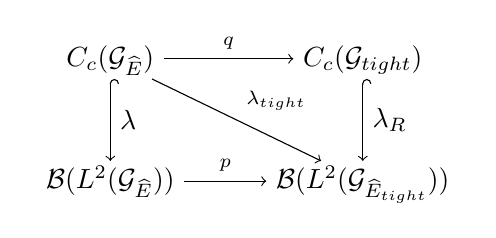
\begin{tikzpicture}
\matrix(m)[matrix of math nodes,row sep=3em, column sep=3em, text height=1.5ex, text depth = 0.25ex]
{C_{c}(\G_{\E})&C_{c}(\G_{tight})\\
\mathcal{B}(L^{2}(\G_{\E}))&\mathcal{B}(L^{2}(\G_{\E_{tight}}))\\};
\path[->,font=\scriptsize]
(m-1-1) edge node[auto] {$q$} (m-1-2)
(m-2-1) edge node[auto] {$p$} (m-2-2)
(m-1-1) edge node[auto] {$\lambda_{tight}$} (m-2-2);
\path[right hook->]
(m-1-1) edge node[auto] {$\lambda$} (m-2-1)
(m-1-2) edge node[auto] {$\lambda_{R}$} (m-2-2);

\end{tikzpicture}
\end{center}

where $\lambda_{R}$ is the left regular representation of $C_{c}(\G_{tight})$. It follows from the definition of $p$ that the bottom triangle commutes and the top triangle commutes as:
\begin{equation*}
\lambda_{x}(f) =\sum_{t \in \Max(S)} f_{t}(x)\lambda_{x}(1_{tt^{*}}\delta_{t}) = \lambda_{x}(qf)
\end{equation*}
For each $x \in \E_{tight}$. Hence:
\begin{equation*}
\Vert qf \Vert_{r} = \sup_{x \in \E_{tight}} \lbrace \Vert \lambda_{x}(qf) \Vert \rbrace = \sup_{x \in \E_{tight}} \lbrace \Vert \lambda_{x}(f) \Vert \rbrace \leq \Vert \lambda(f) \Vert = \Vert f \Vert_{r}
\end{equation*}
and so $q$ is contractive (and therefore continuous).
 
Now to consider (2). It is enough to compute the result of products of elements of the form $f_{s}\delta_{s}$ for some $s \in \Max(S)$. We then check the following two identities:


\begin{enumerate}[I]
\item $q(f_{s}\delta_{s} \Xst f_{t}\delta_{t}) = q(f_{s}\delta_{s})\Xst q(f_{t}\delta_{t})$
\item $(q(f_{s}\delta_{s}))^{*}=q((f_{s}\delta_{s})^{*})$
\end{enumerate}


To see (I) compute on a single element:
\begin{eqnarray*}
(f_{s}\delta_{s} \Xst f_{t}\delta_{t})([st,\phi])=f_{s}(\theta_{t}(\phi))f_{t}(\phi)
\end{eqnarray*}
Apply $q$:
\begin{eqnarray*}
q(f_{s}\delta_{s} \Xst f_{t}\delta_{t})([st,\phi])= (f_{s}\delta_{s} \Xst f_{t}\delta_{t})|_{\E_{tight}}([st,\phi]) =f_{s}(\theta_{t}(\phi))f_{t}(\phi)
\end{eqnarray*}
For all $[st,\phi] \in \G_{\E_{tight}}$. Then compute the right hand side: 
\begin{eqnarray*}
(q(f_{s}\delta_{s}) \Xst q(f_{t}\delta_{t}))([st,\phi])=f_{s}|_{\E_{tight}}(\theta_{t}(\phi))f_{t}|_{\E_{tight}}(\phi)
\end{eqnarray*}
Which matches for each $[st,\phi] \in \G_{\E_{tight}}$. 

To prove (II) we need to compute on a single element, where $(f_{s}\delta_{s})^{*}=\Xlpha_{s^{*}}(\overline{f_{s}})\delta_{s^{*}}$:

\begin{eqnarray*}
q((f_{s}\delta_{s})^{*})([s^{*},x])& = &\Xlpha_{s^{*}}(\overline{f_{s}})_{\E_{tight}}(x)\\
& = & \overline{f}(\theta_{s}(x)) \\ & = & \overline{f(\theta_{s}(x))} \\ & = & \overline{q(f)}(\theta_{s}(x)) \\ & = &  \Xlpha_{s^{*}}(\overline{q(f)})(x)
\end{eqnarray*}
Where the above holds for all $x \in \E_{tight}$ where the function $f_{s}$ is defined at $\theta_{s}(x)$ as required.

As $q$ is a continuous *-homomorphism, it extends to the completions.
\end{proof}

\subsection{Applying the machinery}\label{sect:S1-a}
The following lemma is key in the proof of theorem \ref{thm:PV1}.
\begin{lemma}\label{lem:L3}
Let $S$ be F-inverse and let $K \subset \Max(S)$ such that $K$ is finite and $T=\sum_{t \in K} a_{t}\lambda(1_{tt^{*}}\delta_{t})$ such that $a_{t}$ is the constant function that has value $a_{t}$ on $D_{tt^{*}}$. Then $\Vert T \Vert = \Vert qT \Vert$
\end{lemma}
\begin{proof}
It is immediate that $\Vert T \Vert \geq \Vert qT \Vert$ as $q$ is contractive. We arrive at the other inequality by applying Corollary (\ref{cor:C1}).
\begin{eqnarray*}
\Vert T \Vert_{L^{2}(\mathcal{G}_{x})} = \Vert \sum_{t \in K} a_{t}\lambda_{x}(1_{tt^{*}}\delta_{t}) \Vert = \Vert \sum_{t \in K} a_{t}Q_{x}\lambda_{\infty}(1_{tt^{*}}\delta_{t})Q_{x}^{*} \Vert \\
= \Vert Q_{x}(\sum_{t \in K} a_{t}\lambda_{\infty}(1_{tt^{*}}\delta_{t}))Q_{x}^{*} \Vert = \Vert Q_{x}(qT)Q_{x}^{*} \Vert \leq \Vert qT \Vert.
\end{eqnarray*}
This holds for every $x \in E$ and so by  $\Vert T \Vert = \Vert \lambda(T) \Vert = \sup \lbrace \Vert \lambda_{x}(T) \Vert : x \in E \rbrace \leq \Vert qT \Vert$. This gives the desired equality.  
\end{proof}

We can now state and prove the main result of this section:

\begin{theorem}\label{thm:PV1}
Let $S$ be an F-inverse monoid and let $\G_{\E}$ be its universal groupoid and let $A=C_{c}(\G_{U})$. Then we have the following (intrinsic) short exact sequence of $C^{*}$-algebras:
\begin{equation*}
0 \rightarrow \overline{A} \rightarrow C^{*}_{r}(\mathcal{G}) \rightarrow C^{*}_{r}(G) \rightarrow 0
\end{equation*}
\end{theorem}

\begin{proof}

We know that we have a surjective *-homomorphism $q$ from $C^{*}_{r}(\G)$ to $C^{*}_{r}(G)$, we just need to see that the kernel of this map is $\overline{A}$. The set $\overline{A}$ is contained in the kernel as elements in $A$ are sums of functions with value at $1_{E}=\infty \in \widehat{E}$ of zero and projection onto this value (i.e applying q) will send the entire element to $0 \in C^{*}_{r}(G)$. So it is enough to show that $A$ is dense in the kernel.\\
\\
First consider finite sums. Let $f \in C_{c}(\mathcal{G})$. We need to show that if $qf=0$ then $ f \in A$.\\
\\
$f$ has the form:
\begin{equation*}
f=\sum_{s \in S} f_{s}\delta_{s} \mbox{ } f_{s}\in C(D_{ss^{*}})
\end{equation*}
With only finitely many non-zero terms. This can be viewed concretely on $L^{2}(\mathcal{G})$ using
\begin{equation*}
\lambda(f)=\sum_{s \in S} f_{s}\lambda(1_{ss^{*}}\delta_{s})
\end{equation*}
$S$ F-inverse allows us to reduce this sum using the following observation that for each $s \in S$ we can write the term $f_{s}\delta_{s}$ as $f_{s}\chi_{s}\delta_{t_{s}}$ where $t_{s}$ is the maximal element above $s$. So for each $t \in \Max(S)$ we can define $f^{'}_{t}=\sum_{s \leq t}f(s)\chi_{s}$ and then
\begin{equation}\label{Eq1}
\lambda(f)=\sum_{t \in \Max(S)} f^{'}_{t}\lambda(1_{tt^{*}}\delta_{t})
\end{equation}
(\ref{Eq1}) is in the kernel of $q$ if and only if each $f^{'}_{t}(\infty)=0$ for every $t \in \Max(S)$ that is if and only if $\lambda(f) \in A$.\\
\\
Now let $T$ be an element of $C^{*}_{r}(\G})$ such that $T$ is in the kernel of $q$ ($qT=0$). Then we need to show $T$ can be approximated by finite sums that lie in $A$. Let $T_{n}$ be finite sums in $C_{c}(\mathcal{G})$ with $T_{n} \rightarrow T$. Without loss of generality, these $T_{n}$ have the following form for some finite $K_{n} \subset \Max(S)$:
\begin{equation*}
T_{n}=\sum_{t \in K_{n}} f^{n}_{t}\lambda(1_{tt^{*}}\delta_{t})
\end{equation*}
then $qT_{n} = \sum_{t \in K_{n}} f^{n}_{t}(\infty)\lambda_{\infty}(1_{tt*}\delta_{t})$. Define a pullback of $qT_{n}$:
\begin{equation}
S_{n} = \sum_{t \in K_{n}} a^{n}_{t}\lambda(1_{tt*}\delta_{t}) \in C_{c}(\mathcal{G})
\end{equation}
Where $a^{n}_{t}$ is the constant function on $D_{tt^{*}}$ with value $f_{t}^{n}(\infty)$. It is clear that $qS_{n}=qT_{n}$ and using lemma \ref{lem:L3} we have that $\Vert S_{n} \Vert = \Vert qS_{n} \Vert = \Vert qT_{n} \Vert$ so $\Vert S_{n} \Vert \rightarrow 0$\\
\\
Let $U_{n}=(T_{n}-S_{n})$. Then $U_{n} \in A$ and $U_{n}=(T_{n}-S_{n}) \rightarrow (T-0)=T$, so T can be approximated by elements in $A$, hence $A$ is dense in $ker(q)$.
\end{proof} 
\section{A similar sequence for 0-F-inverse monoids}\label{sect:S2}
In this section we consider a generalisation of Theorem \ref{thm:PV1} to strongly 0-F-inverse monoids with K-exact universal group. First we need some terminology of \cite{MR1911663}.

\begin{definition}
Let $\G$ be an locally compact \'etale groupoid and let $F$ be a subset of the unit space $\G^{(0)}$. We say that $F$ is \textit{saturated} if for all $\gamma \in \G$ with $s(\gamma) \in F$ we also have $r(\gamma)\in F$. 
\end{definition}

Clearly, subsets that are invariant under the action of $S$ are also saturated. The following Lemma outlines the connections between saturation and Morita enveloping actions.

\begin{lemma}\label{Lem:Cut}
Let $\G$ be an \etale locally compact Hausdorff groupoid with a (T,C,F)-cocycle $\rho$ to $\Gamma$. Then relation $\sim$ on $\G^{(0)} \times \Gamma$ preserves saturated subsets of $\G^{(0)}$
\end{lemma}
\begin{proof}
Let $U$ be a saturated subset of $\G^{(0)}$ and let $x \in U$, $y \in U^{c}$. Assume for a contradiction that $(x,g) \sim (y,h)$ in $\G^{(0)} \times \Gamma$. Then there exists a $\gamma$ $\in \G$ such that $s(\gamma)=x$, $r(\gamma)=y$ and $\rho(\gamma)=g^{-1}h$, but as $U$ is saturated no such $\gamma$ exists. 
\end{proof}

\begin{theorem}\label{thm:PV2}
Let $S$ be a strongly $0$-F-inverse monoid with universal group $G:=U(S)$. If $G$ is $K$-exact then the sequence:
\begin{equation*}
0 \rightarrow C^{*}_{r}(\G_{\U}) \rightarrow C^{*}_{r}(\G_{\E}) \rightarrow C^{*}_{r}(\G_{\E_{tight}}) \rightarrow 0
\end{equation*}
is exact at the level of K-theory.  
\end{theorem}
\begin{proof}
We begin by using either Theorem \ref{Thm:IT2-a} or \ref{Thm:IT2} to construct a transformation groupoid $Y_{\E}\rtimes G$ and a Morita equivalence between $\G_{\E}$ and $\Y_{\E}\rtimes G$. We can repeat this process for both $\E_{tight}$ and $U:=\E_{tight}^{c}$, and by Lemma \ref{Lem:Cut} and the fact that quotient maps are open we can conclude that we have a natural sequence of commutative $C^{*}$-algebras:
\begin{equation*}
0 \rightarrow C_{0}(Y_{U}) \rightarrow C_{0}(Y_{\E}) \rightarrow C_{0}(Y_{\E_{tight}}) \rightarrow 0
\end{equation*}
each of which is a $G$-algebra. We now act by the reduced cross product, which produces a sequence of $C^{*}$-algebras:
\begin{equation*}
0 \rightarrow C_{0}(Y_{U})\rtimes_{r}G \rightarrow C_{0}(Y_{\E})\rtimes_{r}G \rightarrow C_{0}(Y_{\E_{tight}})\rtimes_{r}G \rightarrow 0
\end{equation*}
Which may not be exact in the middle term. However, it is exact at the level of K-theory, so consider the K-theory long exact sequence:
\begin{equation*}
\xymatrix@=1em{...\ar[r] & K_{0}(C_{0}(Y_{U})\rtimes_{r} G) \ar[r]& K_{0}(C_{0}(Y_{\E})\rtimes_{r} G) \ar[r]& K_{0}(C_{0}(Y_{\E_{tight}})\rtimes_{r} G)\ar[r] & ...\\
...\ar[r] & K_{0}(C^{*}_{r}(\G_{\U})) \ar[r]\ar[u]^{\ucong}& K_{0}(C^{*}_{r}(\G_{\E})) \ar[r]\ar[u]^{\ucong}& K_{0}(C^{*}_{r}(\G_{\E_{tight}})) \ar[r]\ar[u]^{\ucong}& ...}
\end{equation*}
where the isomorphisms are induced by the Morita equivalences given by Theorems \ref{Thm:IT2-a} and \ref{Thm:IT2}. This concludes the proof.
\end{proof}


\section{Partial Translation Structures.}\label{sect:S3}
In this section we outline the definition of a partial translation structure and describe some of the main results concerning them. Focusing on a special case, what we call \textit{grouplike partial translation structures}, that relates to uniform embeddability into a groups for metric spaces.  We then outline an inverse monoid approach to understanding the translation algebra that can be naturally associated to a partial translation structure.

The concept of a partial translation structure was given in \cite{MR2363428} to study uniform embeddability into groups. By associating to a metric space this additional information, namely a collection of partial bijections that form entourages in the metric coarse structure, you gain control over the local symmetries of the space that preserve metric information. 


\begin{definition}\label{PT2}
A partial translation structure on $X$ is a collection $\mathcal{T}$ of partial translations of $X$ such that for all $R>0$ there exists a finite subset $\mathcal{T}_{R}$ of disjoint partial translations in $\mathcal{T}$ and a collection $\Sigma_{R}$ of partial cotranslations of $\mathcal{T}_{R}$ satisfying the following axioms:
\begin{enumerate}
\item The union of the partial translations  $t \in \mathcal{T}_{R}$ contains the R-neighbourhood of the diagonal.
\item There exists $k$ such that for each $x,x^{'} \in X$ there are at most $k$ elements $\sigma \in \Sigma_{R}$ such that $\sigma x=x^{'}$.
\item For each $t \in \mathcal{T}_{R}$ and for all $(x,y),(x^{'},y^{'}) \in t$ there exists $\sigma \in \Sigma_{R}$ such that $\sigma x=x^{'}$ and $\sigma y=y^{'}$.
\end{enumerate}
\end{definition}

\begin{definition}(Freeness, Global control)
A partial translation structure on X is said to be \textit{free} if in definition \ref{PT2} ii) $k=1$; i.e there is a unique cotranslation such that for each pair $(x,y)\in X \times X$ we have $\sigma x = y$.\\
A partial translation structure on X is said to be \textit{globally controlled} if the partial cotranslation orbits are partial translations. 
\end{definition}

The following lemma is from \cite{MR2363428}.

\begin{lemma}\label{lem:L10}
Let $G$ be a group. $G$ acts on itself on the right by translations. Let $X \subseteq G$ then the restriction of the action of $G$ on itself to the subspace $X$ is a translation structure on $X$ that is free and globally controlled.\qed
\end{lemma}

The intuition for the definition \ref{PT2} is a metric version of a group ``action" for the space, with freeness and global control making the ``action" more like that of a group. (Group actions have these properties, by lemma \ref{lem:L10})

\begin{definition}\label{def:ZD1}
Let $\mathcal{T}$ be a partial translation structure. Then we say $\mathcal{T}$ has \textit{zero divisors} if there exists a product of disjoint translations $t_{1},t_{2},...,t_{n} \in \mathcal{T}$ such that $t_{1}t_{2}t_{3}...t_{n}$ is empty (i.e has empty domain). We say $\mathcal{T}$ has no zero divisors if no such product is empty.
\end{definition}
We specialize our definition slightly in light of the following proposition, the proof of which can be found in \cite[Proposition 8.1]{rosiesthesis}

\begin{proposition}\label{prop:TFAE} Let $G$ be a countable discrete group and let $X \subseteq G$
The following are equivalent:
\begin{enumerate}
\item $X^{c}$ is not coarsely dense in $G$.
\item For every $R>0$ there exists $g \in G$ such that $B_{R}(g) \subseteq X$.
\item The monoid generated by $\mathcal{T}_{G}|_{X}$ has no zero element.
\end{enumerate}
\end{proposition}
The definition provided below is stronger than the definition provided in \cite{MR2363428}, however this better emulates the situation that arises when you consider a space that is uniformly embedded into a group.
\begin{definition}\label{Def:PTS}
Let $X$ be a countable discrete metric space. A collection of partial bijections $\mathcal{T}$ is a called a grouplike partial translation structure for $X$ if:
\begin{enumerate}
\item $\mathcal{T}$ partitions $X\times X$.
\item $\forall t_{i}, t_{j} \in \mathcal{T}$ $\exists t_{k} \in \mathcal{T}$ we have $t_{i}t_{j} \subseteq t_{k}$ (i.e $\mathcal{T}$ is subclosed).
\item $\forall t \in \mathcal{T}$ we have $t^{*} \in \mathcal{T}$.
\item $\mathcal{T}$ has a global identity, denote this $t_{0}$.
\end{definition}

As a consequence of the Wagner-Preston Theorem \cite{MR1455373}, partial bijections move us toward inverse semigroup theory.
\begin{proposition}\label{prop:P6}
Let $X$ be a metric space equipped with a group-like partial translation structure $\mathcal{T}$. Then $\mathcal{T}$ generates an inverse submonoid of $I(X)$
\end{proposition}
\begin{proof}
The axioms for a grouplike structure tell us that for every translation we have the adjoint translation - that acts an inverse. As $\mathcal{T}$ partitions $X \times X#$ we have that for every $t \in \mathcal{T}$ $t^{*}$ is unique. Now these elements are partial bijections on $X$, and so are elements of $I(X)$ - and we can consider the subsemigroup they generate. As each element of this subsemigroup has a unique inverse we get that it must be an inverse subsemigroup. The presence of the global identity map in $\mathcal{T}$ will give a global identity in the subsemigroup it generates. Hence the subsemigroup is a submonoid, as required.
\end{proof}

We can characterise the monoids generated by partial translation structures:

\begin{lemma}\label{Lem:PTS}
The inverse monoid $S$ generated by a partial translation structure $\mathcal{T}$ is 0-F-inverse, with maximal element set $\lbrace t_{i} : t_{i} \in \mathcal{T} \rbrace$. 
\end{lemma}
\begin{proof}
First we prove maximality of the translations. We prove that for any $s\in S \setminus \lbrace 0 \rbrace$ there exists a unique $t \in \mathcal{T}$ such that $s \leq t$. Property (2) from the definition of a translation structure implies that $\mathcal{T}$ generates the partial order on $S$. Property (1) in Definition \ref{Def:PTS}; $\mathcal{T}$ partitions $X \times X$, gives us that for any pair $t_{i},t_{j}\in \mathcal{T}$ $et_{i}=et_{j} \Leftrightarrow t_{i}=t_{j}$. 

Now we prove that $S$ is $0$-E-unitary. Let $e\in E(S)\setminus \lbrace 0 \rbrace$ and $s\in S\setminus \lbrace 0 \rbrace$. Without loss of generality we can treat $s$ as maximal in what follows. Assume that $e \leq s$. This gives us two equations: $es=e \leq s$. As the natural order is preserved by taking inverses we see that $s^{*}e \leq s^{*}$. These imply that $s=s^{*}$. This tells us that $s^{2}$ is idempotent, but we want $s$ idempotent. To show this we will aim for $s^{2}=s^{3}$. Observe that $es=es^{2}\leq s^{2} \leq s$. This implies $s^{2}=fs$ for some $f\in E(S)$. $s^{3}=s^{2}s=(fs)s=f^{2}s=fs=s^{2}$. As $s=s^{3}$ we get $s \in E(S)$ as required.
\end{proof}



\subsection{Translation algebras and a groupoid characterisation.}

Let $X$ be a uniformly discrete bounded geometry metric space.

\begin{definition}
The translation algebra associated with a partial translation structure $\mathcal{T}$ on $X$, denoted by $C^{*}\mathcal{T}$, is the completion as a *-subalgebra of $\mathcal{T}$ viewed as bounded operators on $\ell^{2}(X)$
\end{definition}

The aim of this section is to give a description of the partial translation algebra associated to a grouplike $\mathcal{T}$ with no zero divisors as the $C^{*}$-algebra of a groupoid, where the groupoid is related to the inverse monoid generated by the partial translations. We then recast a result of Brodzki, Niblo, Putwain and Wright Theorem 8.3 \cite{rosiesthesis} outlining a short exact sequence of $C^{*}$-algebras arising from such translation structures and compute some examples in certain cases.

Using Theorem 1 and 2 from \cite{MR2457037} we can draw the conclusion that the left regular representation of $S$ does not generate the correct covariant groupoid representation in general. However it does appear to match in certain cases. To proceed we consider the information we can draw from the underlying space $X$ by extending the representation on $I(X)$, which determines a representation on $\ell^{2}(X)$ in the natural way. This representation will be the focus of this section. The following is Proposition 10.6 \cite{MR2419901}

\begin{proposition}\label{prop:P7} 
Let $\mu$ be a representation of $S$ on a Hilbert Space $H$. Then there exists a unique *-representation $\pi_{\mu}$ of $C_{0}(\E)$ on $H$ such that $\pi_{\mu}(1_{e})=\mu(e)$ for every $e \in E$ In addition $(\pi_{\mu} \times \mu)$ is a covariant representation for $\G_{\E}$. 
\end{proposition}

So given $X$ equipped with a grouplike partial translation structure $\mathcal{T}$, we get an inverse monoid $S=\langle \mathcal{T} \rangle$ and a representation $\mu: S \hookrightarrow I_{b}(X)$ from Proposition \ref{prop:P6}. So applying Proposition \ref{prop:P7} we arrive at a representation $\pi_{\mu}$ of $C(\E)$ on $\ell^{2}(X)$. 

The proof of the below result relies on the spectrum of the commutative $C^{*}$-subalgebra $A=C^{*}_{\pi_{\mu}}(E)$ of $C^{*}_{\mu}(S)\cong C^{*}\mathcal{T}$. We denote the spectrum by $\X$.

\begin{proposition}\label{prop:P9}
If $S$ is as above then the following hold for $\X$:
\begin{enumerate}
\item $\X \hookrightarrow \E$ is a topological embedding
\item $\beta X \twoheadrightarrow \X$ is a quotient map.
\end{itemize}
Moreover the topologies are all compatable with the topology endowed as the spectrum of $A=C^{*}(E)$.
\end{proposition}
\begin{proof}We first give a constructive proof when $S$ has no zero element.
First we show (1). From the proof of Proposition \ref{prop:P7} we see that we have a natural injective continuous map given by: 
\begin{equation*}
j: \psi \in \X \mapsto \phi = \psi \circ \sigma \in \E
\end{equation*}
$j(\X)$ is compact as j is continous and closed because $\E$ is Hausdorff.

It is possible, when $\mathcal{T}$ has no zero divisors, to compute (2) concretely as the quotient map is given by the equivalence relation 
\begin{equation*}
\phi \sim \phi^{'} \leftrightarrow \phi \cap E(S) = \phi^{'} \cap E(S)
\end{equation*}
This map is surjective precisely when given any $\psi \in \X$ we can complete this to an ultrafilter in $\beta X$:
\begin{equation*}
F_{\psi} = \lbrace e \in E(S) | \psi(\sigma(e))=1 \rbrace
\end{equation*}
We can complete this to an ultrafilter in $\beta X$ in many ways (Zorn's Lemma), however it is enough to show we can do it such that $F_{\psi ,UF}\cap E(S) = \psi$. So it is enough to pick subsets according to the following rules. Let $M,M^{c} \in \lbrace 0,1 \rbrace^{X}$ and
\begin{itemize}
\item If $M \in E(S)$ then add $M^{c}$ to $F_{\psi}$
\item If $M \not\in E(S)$ then add $M$ to $F_{\psi}$
\item If $M,M^{c} \not \in E(S)$ add either to $F_{\psi}$
\end{itemize}
With the case in which both $M$ and $M^{c}$ are contained in $E(S)$ is impossible as $E(S)$ has no zero element.

Now $F_{\psi}$ has the correct property and is an ultrafilter of $\beta X$ that maps onto $\psi$. Observe that the image of $\beta X$ is again compact, and thus closed, hence the map is a quotient.

If $\mathcal{T}$ does have zero divisors, the above constructive method will not complete the proof. However, a spectral argument involving $C^{*}$-algebras will. Observe that as each $t_{g}$ is bounded, $C^{*}_{\mu}(S) \subset C^{*}_{u}(X)$ with $C^{*}_{\pi_{\mu}}(E) \subset \ell^{\infty}(X)$. Taking the spectra associated to this inclusion then gives us a map:
\begin{equation*}
r_{\beta X}: \beta X \twoheadrightarrow \widehat{X}
\end{equation*}
which is continuous. In particular as both $\beta X$ and $\widehat{X}$ are compact Hausdorff spaces, this map is closed (and open) and hence a quotient.

In the case that $S$ has a zero element, we appeal to universal properties and another result of Exel \cite{MR2419901}. By Proposition 10.10 \cite{MR2419901} the space $\widehat{X}$ is closed and invariant; we can reduce the universal groupoid $\G_{\E}$ for $S$ to $\widehat{X}$. This we denote by $\G_{\widehat{X}}$. 

Recall each $t \in \mathcal{T}$ is an element of $I_{b}(X)$ implies that the algebra $C^{*}_{\pi}(S)$ is a subalgebra of $C^{*}_{u}X$. We now remark that the representation $\pi_{X}$, when restricted to $C^{*}E$ assigns each idempotent a projection in $C^{*}_{u}X$, that is $C^{*}_{\pi_{X}}(E)=\pi_{X}(C^{*}E) \subset \ell^{\infty}(X)$. Taking the spectra associated to this inclusion then gives us a map:
\begin{equation*}
r_{\beta X}: \beta X \twoheadrightarrow \widehat{X}
\end{equation*}
which is continuous. In particular as both $\beta X$ and $\widehat{X}$ are compact Hausdorff spaces, this map is closed (and open) and hence a quotient. This proof has the upside of working even if $S$ has a zero element, but the downside that it does not explicitly extend the filters in $\X$.
\end{proof}

\begin{corollary}\label{cor:C3}
Let $\psi_{x} = \lbrace x \rbrace^{\uparrow} \cap E(S)$. Then the set $\lbrace \psi_{x} | x \in X \rbrace$ is dense in $\X$.
\end{corollary}

In the most general situation the subspace $X$ may be stabilized under the right or left action of the group; we denote the left stablizer $LStab_{G}(X)$ by $H$. 

\begin{proposition}\label{prop:P9a}
$x_{1}x_{2}^{-1} \in H \Leftrightarrow \forall t \in \mathcal{T} (x_{1} \in Dom(t) \Leftrightarrow x_{2} \in Dom(t))$
\end{proposition}
\begin{proof}
($\Rightarrow$) $x_{1}x_{2}^{-1} \in H$ is equivalent to $x_{1}, x_{2} \in Hx$ for some $x \in X$. This implies that $(x_{1} \in Dom(t) \Leftrightarrow x_{2} \in Dom(t))$ as the elements of $H$ are contranslations of $X$. 

In fact we can say that the elements of $H$ are precisely the cotranslations that are bijections of $X$. This is key in proving the converse:

($\Leftarrow$) Consider $h=x_{1}x_{2}^{-1}$. We want to see that for all $x \in X$ $hx \in X$. Observe that by the first property of translation structures there exists a unique translation $t$ such that $t(x_{2})=x$ Then $hx=ht(x_{2})=t(hx_{2})=t(x_{1}) \in X$ and this chain of equalities holds precisely when $(x_{1} \in Dom(t) \Leftrightarrow x_{2} \in Dom(t))$

\end{proof}

\begin{corollary}\label{cor:C5}
$B$ is in bijection with $H \backslash X$
\end{corollary}
\begin{proof}
The righthand side of Proposition \ref{prop:P9a} is equivalent to the condition that $\psi_{x_{1}}=\psi_{x_{2}} \in B$.
\end{proof}

It is immediate (using \cite[Prop 10.10]{MR2419901}) that the set $\X$ is invariant under the action of $S$. To compute the groupoid and groupoid $C^{*}$-algebras associated to $\X$ we would like to know a little more about the Hilbert spaces associated to the fibers and general connectness of the set $B:=\lbrace \psi_{x} | x \in X \rbrace$ (which using Corollary \ref{cor:C3} is dense in $\X$).

\begin{proposition}\label{prop:P10}
Let $t \in \mathcal{T}$. Then $\theta_{t}(\psi_{x})=\psi_{t(x)}$ for all $x \in Dom(t)$.
\end{proposition}
\begin{proof}
First some observations:
\begin{enumerate}
\item $\theta_{t}(\psi_{x})$ is defined as $\theta_{t}(\psi_{x}) \in D_{tt^{*}} \Leftrightarrow \psi_{x} \in D_{t^{*}t} \Leftrightarrow t^{*}t \in \psi_{x} \Leftrightarrow x \in t^{*}t = Dom(t)$.
\item $(\theta_{t}(\psi_{x}))(tet^{*})=\psi_{x}(t^{*}(tet^{*})t)=\psi_{x}(e)$. Hence $e \in \psi_{x} \Leftrightarrow tet^{*}  \in \theta_{t}(\psi_{x})$.
\item $\psi_{x}=\psi_{y} \Leftrightarrow \psi_{t(x)}=\psi_{t(y)}$, in fact more is true as: $\psi_{t(x)}=\psi_{t^{'}(y)} \Leftrightarrow Dom(t^{'})=Dom(t)$.
\end{enumerate}
We prove inclusions. First $\theta_{t}(\psi_{x}) \subset \psi_{t(x)}$. Without loss of generality, we can take $tet^{*}$ to be the general form of an element of $\theta_{t}(\psi_{x})$ and then: $tet^{*} \in \psi_{t(x)} \Leftrightarrow t(x) \in tet^{*} \Leftrightarrow tet^{*}(t(x))=t(x)$, which is the case if and only if $e \in \psi_{x}$.

To see the reverse inclusion let $f \in \psi_{t(x)}$. Then $f \in \theta_{t}(\psi_{x}) \Leftrightarrow t^{*}ft \in \psi_{x} \Leftrightarrow t(x) \in f \Leftrightarrow f \in \psi_{t(x)}$. 

To conclude; (3) controls the behavior of the action when the stabilizer is non-trivial, the first part shows the action behaves with respect to the quotient and the second part shows that given any pair $(x^{'},y^{'})\in X \times X$ such that $x^{'}\in Hx, y^{'}\in Ht(x)$ the unique translation $t_{x^{'}y^{'}} \in \mathcal{T}$ that sends $x^{'}$ to $y^{'}$ defines an arrow between $\psi_{x}$ and $\psi_{t(x)}$. 
\end{proof}

\begin{proposition}\label{cor:C4}
$B$ is invariant and $\G_{B}$ is connected. Moreover if $H$ is trivial, then $B$ is invariant and $\G_{B}$ is uniquely connected.
\end{proposition}
\begin{proof}
$B$ is invariant as a consequence of Proposition \ref{prop:P10}, and connected by the first property of grouplike partial translation structures - $\mathcal{T}$ partitions $X \times X$. This tells us that when we pass to the quotient $H \backslash X$ we get a collection of arrows between each pair of points that are indexed by $H$. 

In the situation that $H$ is trivial we get a unique arrow between any two points in $B$ and $B$ is in bijection with $X$, hence the groupoid $\G_{B}$ is precisely the pair groupoid $X \times X$, with the norm coming from the stalks, each of which have the form of $\ell^{2}(X)$ by the uniquely connected property of $B$.
\end{proof}

\begin{remark}
In the situation that $H$ is non-trivial, we have a unit space for $\G_{B}$ that is $B\times B$, with arrows between each pair indexed by $H$. The Hilbert space associated to each fibre $L^{2}(\G_{\X})|\psi_{x}$ is exactly the Hilbert space with basis indexed by the \textit{arrows} $[t_{h},\psi_{x}]$ - the set of arrows based at $\psi_{x}$ is in bijection with $X$, construct a map using the first property of translation structures.

For each point $hx \in Hx$ there exists a unique translation $t_{y,h}$ to each other point $y \in X$. We then define the map $[t_{y,h}, \psi_{x}] \mapsto t_{y,h}(hx)=y$.

This provides a unitary isomorphism between these spaces, denote this map at the level of Hilbert spaces by $U_{x}$ for each $x \in H \backslash X$.
\end{remark}

\begin{lemma}\label{prop:P11}
$\Vert \lambda(1_{tt^{*}}\delta_{t}) \Vert = \Vert \mu(t) \Vert_{\ell^{2}(X)}$ for all $t \in \mathcal{T}$. 
\end{propositon}
\begin{proof}
The proof of this fact follows from a computation on the basis of $\ell^{2}(X)$ using the unitary isomorphism $U_{x}$. We compute $U_{x}\lambda_{\psi_{x}}(1_{tt^{*}}\delta_{t})U_{x}^{-1}$ evaluated on a basis element $\delta_{y} \in \ell^{2}(X)$.
\begin{enumerate}
\item $U_{x}^{-1}(\delta_{y})=\delta_{[t_{y,h},\psi_{x}]}$
\item $\lambda_{\psi_{x}}(1_{tt^{*}}\delta_{t})(\delta_{[t_{y,h},\psi_{x}]})(\delta_{[s,\psi_{x}]})=\sum_{\substack{[n,\psi_{z}][u,\psi_{x}]\\=[s,\psi_{x}]}} 1_{tt^{*}}([n, \psi_{z}]\delta_{[t_{y,h},\psi_{x}]}([u,\psi_{x}])=\delta_{[t_{y,h},\psi_{x}]}$

Hence $\lambda_{\psi_{x}}(1_{tt^{*}}\delta_{t})$ moves the basis element $\delta_{[t_{y,h},\psi_{x}]}$ to the basis element $\delta_{[s,\psi_{x}]}$, where $s$ is the unique translation above $tt_{y,h}$ in $\mathcal{T}$. This is summarized in figure \ref{}.
\item $U_{x}(\delta_{[tt_{y,h},\psi_{x}]})=\delta_{t(t_{y,h}(hx))}=\delta_{t(y)}=\mu(t)(\delta_{y})$.
\end{enumerate}
This holds for all $y$ in the domain of $t$, as the multiplication in the groupoid is defined for only that situation.

As we have this equality for each $\psi_{x} \in B$; we get that $\Vert \lambda(1_{tt^{*}}\delta_{t}) \Vert_{r} = \sup \lbrace \Vert \lambda_{\psi_{x}}(1_{tt^{*}}\delta_{t}) \Vert : \psi_{x} \in B \rbrace = \Vert \mu(t) \Vert_{\ell^{2}(X)}$.
\end{proof}
\end{proposition}

This extends to finite sums:

\begin{lemma}\label{lem:L7}
Let $K \subset \X$ be a finite subset and let $a_{t}$ be the constant function valued $a_{t}$ on $D_{tt^{*}}$. Then \Vert \sum_{t \in K} a_{t}\delta_{t} \Vert_{r} = \Vert \sum_{t \in K} a_{t} \mu(t) \Vert_{\ell^{2}(X)}  
\end{lemma}
\begin{proof}

First we show that $\sum_{t \in K} a_{t}\delta_{t}$ represents as $\sum_{t \in K} a_{t} \mu(t)$ on the basis of $\ell^{2}(X)$. We proceed as in proposition \ref{prop:P10}. 

First compute $U_{x}^{-1}(\delta_{y})$:
\begin{equation*}
U_{x}^{-1}(\delta_{y})=\delta_{[t_{y,h},\psi_{x}]}
\end{equation*}
Then compute: 
\begin{eqnarray*}
(\sum_{t \in K}\lambda_{\psi_{x}}(a_{t}\delta_{t}))(\delta_{[t_{y,h},\psi_{x}]})& = &\sum_{\left\lbrace t\in K:\substack{[t,\psi_{y}][t_{y,h},\psi_{x}]\\=[tt_{y,h},\psi_{x}] }\right\rbrace} a_{t}([t, \psi_{y}])\delta_{[t_{y,h},\psi_{x}]}([t_{y,h},\psi_{x}])\\
& = &\sum_{\lbrace t \in K, y \in Dom(t)\rbrace }a_{t}([t,t_{y,h}(\psi_{x})])\delta_{[tt_{y,h}, \psi_{x}]}\\ & = &\sum_{t \in K,y \in Dom(t)}a_{t}\delta_{[tt_{y,h}, \psi_{x}]}
\end{eqnarray*}
Lastly move back to $\ell^{2}(X)$ via $U_{x}$:
\begin{eqnarray*}
U_{x}(\sum_{t \in K,y \in Dom(t)}a_{t}\delta_{[tt_{y,h}, \psi_{x}]}) & = &\sum_{t \in K, y \in Dom(t)}a_{t}\delta_{t(y)}\\ & = &(\sum_{t \in K}a_{t}\mu(t))(\delta_{y})
\end{eqnarray*}

\end{enumerate}

So both finite sums transform the basis in the same way. This equality holds for each $\psi_{x}$ in $B$, so we can conclude that $\Vert \sum_{t \in K} a_{t}\delta_{t} \Vert_{r} = \sup \lbrace \Vert \lambda_{\psi_{x}}(\sum_{t \in K} a_{t}\delta_{t} ) \Vert : \psi_{x} \in B \rbrace = \Vert \sum_{t \in K} a_{t} \mu(t) \Vert_{\ell^{2}(X)}$.
\end{proof}

This lets us define a map: 
\begin{equation*}
\mathcal{Q}: \lambda(1_{tt^{*}}\delta_{t}) \mapsto \mu(t)
\end{equation*}

Now we can state the main result of this section:
\begin{theorem}\label{thm:T5}
Let $X \subset G$, giving us a translation structure $\mathcal{T}_{G}|_{X}$ with no zero divisors and a representation $\mu: S = \langle \mathcal{T}_{G}|_{X} \rangle$. Then we have an isomorphism C^{*}_{r}(\G_{\X}) \cong C^{*}_{\mu}(S) = C^{*}\mathcal{T}. 
\end{theorem}

\begin{proof}
The map $\mathcal{Q}$ is surjective onto $\mathbb{C}S$ (mapping to the generators of $S$), so it remains to see that it passes to the completion and is injective. 
To show this, we appeal to Lemma \ref{lem:L7} to show that the norms match under the map $\mathcal{Q}$ up to finite sums - making the map on the incomplete algebras uniformly continous. Ideally, we would now complete - however we need to be careful as the incomplete *-algebra $M$ generated by finite sums of $1_{e}\delta_{t}$ may not be dense (and is the source of the map $\mathcal{Q}$).

To get over this obstruction we observe that by Stone-Weierstrass every element in $C(\X)$ can be approximated by elements of the form $1_{e}$, i.e for all $f_{t} \in C(\X)$:
\begin{equation*}
f_{t} = \lim_{n} (\sum_{e \in E} a^{n}_{e}1_{e})
\end{equation*}
So for a particular element  $f=\sum_{t \in K}f_{t}\delta_{t} \in C_{c}(\G_{\X})$ we can approximate each $f_{t}$ in turn by limits of $\sum_{e \in E} a_{e}1_{e}$ giving us an approximation by finite sums of elements in $M$. Hence $\overline{M} = C^{*}_{r}(\G_{\X})$, allowing $\mathcal{Q}$ to pass to completions (by uniform continuity).

After passing to the completion, the map is isometric; hence injective. This gives us the first isomorphism. To see the equality, observe that by definition the translation algebra is the algebra generated in $\mathcal{B}(\ell^{2}(X))$ by the set of operators $\lbrace \mu(t) | t \in \mathcal{T} \rbrace$. This is precisely $C^{*}_{\mu}(S)$.
\end{proof}

In this situation we still have access to all the tools available in the general inverse monoid case, as well as all the geometric properties arising from the representation $\mu$.

\begin{corollary}\label{thm:T4}
Let $X \subset G$, $\mathcal{T}=\mathcal{T}_{G}|_{X}$ be a grouplike partial translation structure on $X$ with no zero divisors and $S=\langle \mathcal{T} \rangle \hookrightarrow_{\mu} I(X)$ be the associated F-inverse monoid. Then we have the following (intrinsic) short exact sequence of $C^{*}$-algebras:
\begin{equation}\label{eqn1}
0 \rightarrow C^{*}_{r}(\G_{U}|_{\X}) \rightarrow C^{*}_{r}(\G_{\X}) \rightarrow C^{*}_{r}(G) \rightarrow 0
\end{equation}
Where the middle term is the translation algebra associated to $X$ arising from $\mathcal{T}$
\end{corollary}
\begin{proof}
The proof follows the same lines as the proof of Theorem \ref{thm:T1}.
\begin{enumerate}
\item The map defined on finite sums still has the desired properties, i.e a finite sum is in the kernel if and only if all its components are 0.
\item We still have the same pullbacks of constant functions to the entire space; This enables the same construction of approximating elements; who each have the same norm control property provided by corollary \ref{cor:C1}.
\item We can then conclude that the kernel is the desired algebra (by density).
\end{enumerate}
\end{proof}

Using Theorem \ref{thm:PV2} we can additionally prove the 0-ed analogue of Corollary \ref{thm:T4}:

\begin{corollary}\label{cor:T4}
Let $X \subset G$, $\mathcal{T}=\mathcal{T}_{G}|_{X}$ be a grouplike partial translation structure on $X$ and $S=\langle \mathcal{T} \rangle \hookrightarrow_{\mu} I(X)$ be the associated strongly 0-F-inverse monoid. Then we have the following (intrinsic) short exact sequence of $C^{*}$-algebras:
\begin{equation*}
0 \rightarrow C^{*}_{r}(\G_{U}|_{\X}) \rightarrow C^{*}_{r}(\G_{\X}) \rightarrow C^{*}_{r}(\G_{\E}|_{\X\cap\E_{tight}}) \rightarrow 0
\end{equation*}
\end{corollary}

Even though Corollary \ref{thm:T4} is a consequence of Corollary \ref{cor:T4} the former is more in keeping with the spirit of the original work of Pimsner and Voiculescu and is more directly useful in the computations present in Section \ref{sect:K-theory}.

\section{Applications to coarse geometry and operator K-theory of group $C^{*}$-algebras.}\label{sect:S4}

In this section we construct some examples, some well known in the literature, of inverse monoids associated to subspaces of groups. We then consider applications of the results outlined in the previous sections of the paper combined with a result of Norling concerning the K-theory of $C^{*}_{r}(S)$, when $S$ is stonrgly 0-F-inverse. We first begin with a seemingly disconnected topological notion:

\begin{definition}
Let $X$ be a totally disconnected space. A set $\mathcal{V}$ is said to be a \textit{regular basis} for the topology of $X$ if:
\begin{enumerate}
\item $\mathcal{V}\cup \lbrace \emptyset$ is closed under finite intersections; 
\item $\mathcal{V}$ generates the compact open sets of $X$;
\item $\mathcal{V}$ is independent, that is for every finite family $X,X_{1},...,X_{n} \in \mathcal{V}$ such that $X = \cup_{i=1}^{n} X_{i}$ there exists an $i \in \lbrace 1,..,n \rbrace$ such that $X=X_{i}$.
\end{enumerate}
\end{definition}

In \cite{CEL-2} the authors compute the K-theory for transformation groupoid $C^{*}$-algebras associated to actions of discrete groups $G$ on totally disconnected spaces $\Omega$ that carry a regular $G$-invariant basis. They rely on the Baum-Connes conjecture to deal with certain coefficient algebras via KK-theory. Furthermore, in \cite{Nor-2012}, Norling gave a proof that the basis $\lbrace \widehat{D}_{e} | e \in E \rbrace$ associated to a strongly $0$-F-inverse monoid $S$ is a regular basis of $\E$, and that the induced basis of $Y_{\E}$ is also regular and $G$-invariant. To compute the K-theory requires an understanding of the following equivalence relation:

\begin{definition}
Let $e,f \in E(S)$. $e \approx f$ if $\exists s \in S$ such that $e \leq s^{*}s$ and $ses^{*}=f$.
\end{definition}

This equivalence relation captures information about the action of $S$ on its idempotents $E$, which is naturally used to construct the basis elements $D_{e}$ and the groupoid $\G_{\E}$, hence is intimately connected to the structure of $C^{*}_{r}(S)$. The main result of \cite{Nor-2012}, which utilises this relation, is stated below:

\begin{theorem}\label{Thm:Norling}
Let $S$ be a strongly 0-F-inverse monoid with universal group $G$, where $G$ has the Haagerup property. Then there is an isomorphism:
\begin{equation*}
K_{*}(C^{*}_{r}(S)) \cong \bigoplus_{[e]\in \frac{E^{\times}}{\approx}} K_{*}(C^{*}_{r}(G_{e})
\end{equation*}
Where $G_{e}$ is the stabiliser, in the conjugation action of $S$ on $E$, of the idempotent $e$
\end{theorem}

This Theorem gives a method for computing the K-theory for certain reduced semigroup $C^{*}$-algebras, in particular those constructed from partial translation structures arising from groups. We consider some general natural inverse monoids and compute both the K-theory groups and the associated long exact sequence that arises from the corresponding Pimnser-Voiculescu type sequence.

\subsection{K-theory examples.}\label{sect:K-theory}

\begin{example}\label{Ex:Toe}(Toeplitz extension)
Let $X=\mathbb{N} \subset \mathbb{Z}=G$. We arive at a partial translation structure for $X$ by considering the maps:
\begin{eqnarray*}
& t_{n}: \mathbb{N} \rightarrow \mathbb{N}, x \mapsto x+n \\
&t_{-n}: \mathbb{N} \rightarrow \mathbb{N}\setminus \lbrace 0,1,...,n-1 \rbrace , x \mapsto x-n
\end{eqnarray*} 
These partial bijections generate an inverse monoid, given by the presentation:
\begin{equation*}
S=\langle t_{n},t_{n}^{*}=t_{-n} | t_{n}^{*}t_{n}=1 \rangle
\end{equation*}
This is a well known example from semigroup theory called the \textit{Bicyclic Monoid}. It is well known also that the translation algebra is the universal algebra generated by a unilateral shift; the Toeplitz algebra. To understand the translation algebra, it is enough to compute $\X$. We know that $\X$ is the quotient of $\beta \mathbb{N}$ using the family of domains of the maps $t_{n}$ as $n$ runs though $\mathbb{Z}$, which are in particular cofinite.

\begin{claim}\label{prop:example}
If $E(S) \subseteq $ Cofin($X$) then $\X = (H \backslash X)^{+}$   
\end{claim}
\begin{proof}
It is enough to remark that in general we have:
\begin{equation*}
\X = H\backslash X \cup {1_{E}} \cup \lbrace \mbox{Filters arising from nonprincipal ultrafilters in } \beta X \rbrace
\end{equation*} If we assume $E(S) \subseteq $ Cofin($X$) then \textit{all} nonprincipal ultrafilters will agree in the quotient as they only fight over (and subsequently differ on) infinite subsets with infinite compliments.
\end{proof}

In this example the stabilizer $H$ is trivial, so $\X = \mathbb{N}^{+} = \E$. So we have that the quotient map $C^{*}_{r}(\G_{\E}) \rightarrow C^{*}_{r}(\G_{\X})$ is the identity and the (groupoid) translation algebra is also the Toeplitz algebra.

We remark that Theorem \ref{Thm:Norling} of Norling now gives a direct computation of the K-groups in this instance, as each idempotent is related to $1$ via the translation that sends $1$ to $n$ for each $n$. So it is enough to understand the stabiliser group $G_{1}$, which in this instance is trivial. Hence we get that the K-theory groups are those of a point, which is well-known although computed in a different manner \cite{MR587369,MR2457037}.
\end{example}

\begin{example}(Bridget-Rhodes expansion of a group)
In this instance there is much more interesting K-theory arising from Theorem \ref{Thm:Norling}. The Bridget-Rhodes expansion of a group \cite{MR745358,MR2221438} was first outlined in Section \ref{sect:BRE} as an example. We recall the construction again for clarity.

In the context of a group $G$ we define an a set $S(G)$, the elements are given by pairs: $(X,g)$ for $\lbrace 1,g\rbrace \subset X$, where $X$ is a finite subset of $G$. The set of such $(X,g)$ is then equipped with a product and inverse:
\begin{equation*}
(X,g)(Y,h) = (X\cup gY,gh)\mbox{ , } (X,g)^{-1}=(g^{-1}X,g^{-1})
\end{equation*}
This turns $S(G)$ into a inverse monoid with maximal group homomorphic image $G$, satisfying a universal covering property for partial $G$-actions. The partial order on $S(G)$ can be described by reverse inclusion, induced from reverse inclusion on finite subsets of $G$. It is F-inverse, with maximal elements: $\lbrace(\lbrace 1,g \rbrace, g):g \in G \rbrace$. 

Using Theorem \ref{Thm:Norling}, provided the group has the Haagerup property, we can again compute the K-theory, each finite subset $F$ of $G$ containing $1$ admits the partial action by the group elements that arise within the finite subset; any finite subgroup occurs this way and this gives us all the possible stabilisers. Denote the subset of finite subgroups by $FSG(G)\subset Fin(G)_{1}$. 

The main outcome of this is the following calculation:

\begin{equation*}
K_{*}(C^{*}_{r}(S)) \cong \bigoplus_{\substack{[F] \\ F \in Fin(G)_{1}}} K_{*}(C^{*}_{r}(G_{F})) \cong \bigoplus_{\substack{[F] \\F \in FSG(G)^{c}} }\mathbb{Z} \oplus \bigoplus_{\substack{[F] \\F \in FSG(G) }}K_{*}(C^{*}_{r}(F))
\end{equation*}

In the light of Theorem \ref{thm:PV1} this suggests it should be possible, using the long exact sequence, to compute the K-theory of $C^{*}_{r}(G)$ from information about its finite subgroups.

If $G$ is finite then it appears as an element in $FSG(G) \subset Fin(G)_{1}$ and so the sequence provided by Theorem \ref{thm:PV1} will split at the level of K-theory. Additionally, if we assume $G \cong C_{p}$, the cyclic group of order $p$ for some prime $p$ it is possible to compute the size of the index sets that occur. For each $n$, the number of elements of $Fin(C_{p})_{1}$ of cardinality $n$ is ${p-1 \choose n}$ and so the cardinality of $E(S)$ will be $\sum_{n\geq 1} {p-1 \choose n-1} = F_{p-1}$ the $p-1$ term in the Fibonacci sequence. 

To compute the index we need to know how many of these are related via the partial action of $C_{p}$ and each subset of cardinality $n$ can be related to $n$ other elements: hence the number of orbits of subsets of size $n$ is precisely $\frac{1}{n} {p-1 \choose n-1}$. Let $k_{p}:= 1+ \sum_{n>0}\frac{1}{n} {p-1 \choose n-1}$ Hence we get:

\begin{equation*}
K_{*}(C^{*}_{r}(S(C_{p})) \cong \bigoplus_{k_{p}}\mathbb{Z} \oplus K_{*}(C^{*}_{r}(C_{p}))
\end{equation*}

We remark that it is possible to arrive at this inverse monoid in a natural way via a subset of a group known as a universal deep set \cite{BNW-KTA}. This subset is universal for partial translation structures, and that it generates this inverse monoid is immediate.

\end{example}

We now shift our considerations to the free group on two generators. In this setting, it is possible to get inverse monoids coming from translation structures that are richer in interesting behaviour. We outline some of their natural properties:

\begin{claim}
Let $X \subset F_{2}$ be connected and let $g$ and $h$ be words in $F_{2}$ such that $gh$ contains no $a_{i}a_{i}^{-1}$ or $a_{i}^{-1}a_{i}$. Then the the translations $\lbrace t_{g} | g \in F_{2} \rbrace$ satisfy $t_{g}t_{h}=t_{gh}$. 
\end{claim}
\begin{proof}
These translations differ only by the fact that the product $t_{g}t_{h}$ may contain a relation that is unreduced, whereas $t_{gh}$ acts by the reduced form of $gh$. As there are no relations other than $a_{i}a_{i}^{-1}$ or $a_{i}^{-1}a_{i}$ in $F_{2}$ whence $t_{g}t_{h}$ and $t_{gh}$ agree everywhere they are defined.
\end{proof}

This property makes working with translation algebras arising from $F_{2}$ easier.

\begin{example}\label{ex:PV}(A free group via the Pimsner-Voiculescu method)
Let $X$ be the subset of the free group $F_{n}=\langle a_{1},...,a_{n} \rangle$ consisting of all the words that do not start with an $a_{1}^{-1}$. This subset was considered in \cite{MR670181} and gave rise to a short exact sequence:
\begin{equation*}
0 \rightarrow \mathcal{K}(\ell^{2}(X)) \rightarrow C^{*}\mathcal{T}_{n} \rightarrow C^{*}_{r}F_{n} \rightarrow 0.
\end{equation*}
This sequence is the translation algebra sequence that arises from Theorem \ref{thm:T4}. In addition to this sequence the authors of \cite{MR670181} gave a computation of the K-theory groups associated to $C^{*}\mathcal{T}_{n}$ as those for $C^{*}_{r}F_{n-1}$, giving an inductive method for computing the K-theory of a free group $C^{*}$-algebra. We give a new proof using the generalised short exact sequence from Theorem \ref{thm:PV1} and Theorem \ref{Thm:Norling}.

For this subspace the behavour is exceptionally like the Toeplitz shift in Example \ref{Ex:Toe}, however it is decidedly more complex than in that instance.

\begin{claim}
Let $w \in F_{n}$. Then $t_{w}^{*}t_{w}\approx 1$.
\end{claim}
\begin{proof}
We will prove this by induction on the length of $w$. This clearly holds for the case when the length of $w$ is $1$. So now, assume this holds for length equal to $n$ and let $w$ have length $n+1$. Consider $t_{w}^{*}t_{w}$; this will be a word of length $2n+2$ containing a relation of the form in the centre $t_{a_{i}^{\pm 1}}^{*}t_{a_{i}^{\pm 1}}$ for some $i$. If $i$ is not 1, and this word is not $t_{a_{1}}t_{a_{1}}^{*}$ then we can reduce the idempotent in length to $2n$, represented by the word $w_{1}$ with left end removed. So, we can suppose that the centre of $t_{w}^{*}t_{w}$ is $t_{a_{1}}t_{a_{1}}^{*}$. Now, if the outer translation is a $t_{a_{i}^{\pm 1}}$ for $i$ not $1$, then it is a bijection, and we can apply this bijections inverse without disrupting the equivalence relation $\approx$. This again reduces the length of the word by $1$. Finally, suppose that $w$ starts and ends with $a_{1}^{-1}$. Then $t_{w}^{*}t_{w}$ is certainly less than $t_{a_{1}}t_{a_{1}}^{*}$, at which point we can conjugate by $t_{a}$, preserving the relation $\approx$ and reducing our idempotent in length by $2$. 
\end{proof}

This however doesn't let us compute for a general $e$, which will be a product of conjugates of the $t_{w}^{*}t_{w}$.

Putting this together with the long exact sequence in K-theory connecting the short exact sequences from Theorem \ref{thm:PV1} and Theorem \ref{thm:T4} gives us the following diagram of K-theory groups:

$$
\xymatrix@=0.7em{\ar[r] & 0 \ar[r]\ar[d] & K_{0}(C^{*}_{r}(\G_{U\cap \widehat{X}^{c}}))\ar[d] \ar[r]^{\cong}& K_{0}(\ker p) \ar[r]\ar[d]& 0 \ar[r]\ar[d] & K_{1}(C^{*}_{r}(\G_{U\cap \widehat{X}^{c}})) \ar[r]\ar[d]^{\ucong} &\\
\ar[r] & K_{1}(C^{*}_{r}(F_{n})) \ar[r]\ar[d]^{\ucong} & K_{0}(C^{*}_{r}(\G_{U}))\ar[r]\ar[d]& K_{0}(C^{*}_{r}(F_{n-1})) \oplus \bigoplus_{[ef]_{\approx}} K_{*}(\mathbb{C})\ar[r]\ar[d]^{p}& K_{0}(C^{*}_{r}(F_{n}))\ar[r]\ar[d]^{\ucong} & K_{1}(C^{*}_{r}(\G_{U}))\ar[d] \ar[r] & \\
\ar[r] & K_{1}(C^{*}_{r}(F_{n})) \ar[r]& K_{0}(\mathcal{K}(\ell^{2}(X))) \ar[r]& K_{0}(C^{*}\mathcal{T}_{n}) \ar[r]& K_{0}(C^{*}_{r}(F_{n})) \ar[r]& 0 \ar[r] & 
}
$$

This indicates that whilst the translation algebra $C^{*}\mathcal{T}_{n}$ does not have the same K-theory as $C^{*}_{r}(S)$, the K-theory sequence is split (this relies on the results of Pimsner-Voiculescu \cite{MR670181}: $K_{*}(C^{*}\mathcal{T}_{n}))\cong K_{*}(C^{*}_{r}(F_{n-1}))$), so we are picking out the correct K-theory group as well as much more complex information that comes from the product structure on the idempotents. This is connected to regularisation of the generating set for the basis of $\E$, and will be discussed later in the section.

\begin{example}(Polycyclic monoids, Strong orthogonal completions and the Cuntz extension)
Let $X$ be the set of all the positive words within the free group $F_{n}$. We consider the inverse monoid that arises from the induced translation structure. In this case the inverse monoid has a zero element and satisfies the relations: $t_{a_{i}}^{*}t_{a_{j}}=\delta_{ij}$, $t_{a_{i}}t_{a_{i}}^{*} \leq 1$. The inverse monoid satisfying this relation is called the \textit{polycyclic monoid} \cite{MR1694900,MR2372319,lawson-2011-1, MR1724106}, which is a generalisation of the Bicyclic monoid. We denote this inverse monoid by $P_{n}$.


In this case, we again have that $E(P_{n})$ is in bijection with $X$, which is a rooted binary tree. Hence $\E(P_{n}) \cong \X$. However, many of the domains of translation are infinite with infinite compliment and so we have nontrivial ultrafilters to consider. In general we should consider tight filters, as the closure of the ultrafilters, but by work of Lawson \cite{lawson-2011-1} $P_{n}$ is compactible for each $n$, that is the ultrafilters are closed in the subspace topology on $\E$. As a free group is exact, we can appeal to Theorem \ref{thm:PV2} to get a short exact sequence:
\begin{equation*}
0 \rightarrow C^{*}_{r}(\G_{U}) \rightarrow C^{*}_{r}(\G_{\E}) \rightarrow C^{*}_{r}(\G_{\E_{\infty}}) \rightarrow 0.
\end{equation*}
We would like to understand the algebras that appear within this sequence. Let us begin with the first term; as the left stabiliser of this subspace is trivial we can deduce from Proposition \ref{cor:C4} that $\G_{U}$ is a pair groupoid, hence $C^{*}_{r}(\G_{U})$ is the compact operators on $\ell^{2}(X)$. The middle term satisfies the relation $\sum_{i=1}^{n}t_{a_{i}}t_{a_{i}}^{*} \leq 1$, whence $C^{*}_{r}(\G_{\E}) \cong C^{*}_{r}(S)$ admits a map to $E_{n}$, the generalised Cuntz algebra. It is well known that this map is an isomorphism \cite{MR1724106,MR584266}. It now follows that $C^{*}_{r}(\G_{\E_{\infty}})$ is isomorphic to the Cuntz algebra $\mathcal{O}_{n}$.

We again appeal to Theorem \ref{Thm:Norling} to compute the K-theory. By Proposition \ref{prop:P10} we know that the action on $E(P_{n})$ translates, via the bijection onto $X$, to the translation action of $F_{n}$ on $X$. It follows that there is only a single orbit under this action as partial translation actions are transitive. The stabiliser is obvious trivial in this case, hence by Theorem \ref{Thm:Norling} we arrive at the computation $K_{*}(C^{*}_{r}(P_{n})) \cong K_{*}(\mathbb{C})\cong \mathbb{Z}$. All that remains is to compute the maps in the sequence, which are also well known..

We give a direct computation of the K-theory of the final term here, by considering Lawsons \textit{orthogonal completions} of $P_{n}$ \cite{lawson-2011-1}, denoted by $D(P_{n})$ and $C(P_{n})$ respectively.

\begin{definition}
Let $E$ be a semilattice and let $e,f \in E$. $e$ is \textit{dense} in $f$ if $e \leq f$ and there does not exist $z \in E$ such that $z \leq f$ and $ze=0$. 
\end{definition}

We remark that any tight representation of a inverse monoid cannot separate dense idempotents \cite{MR2419901}. This is particularly relevent in this example. It is clear that in $P_{n}$ the elements $\lbrace t_{a_{i}}t_{a_{i}}^{*} | i = 1,..,n \rbrace$ are pairwise orthogonal, and in the reduced $C^{*}$-algebra they have sum that is less than $1$. The idea of the orthogonal completion is to capture this $C^{*}$-algebraic behavour in an inverse monoid; in $D(P_{n})$ the sum $\bigvee_{i=1}^{n} t_{a_{i}}t_{a_{i}}^{*}$ is defined and is dense in $1$, and equal to $1$ in $C(P_{n})$, which has an underlying tight representation of $S$. 

It follows, from von Neumann equivalence of projections, that each $t_{a_{i}}t_{a_{i}}^{*}$ viewed as an operator in $C^{*}_{r}(\G_{\E_{\infty}})$ is equivalent to $1$ at the level of K-theory, in paricular using Proposition 5.3.1 and Lemma 5.3.2 from \cite{MR1222415} we observe that $C^{*}_{r}(\G_{\E_{\infty}})$ is stable and that $[1]=\sum_{i=1}^{n}[1]$. From above, we know that the K-theory group $K_{0}(C^{*}_{r}(P_{n}))$ is generated by the class $[1]$, hence we know that $[1]$ generates $K_{0}(C^{*}_{r}(\G_{\E_{\infty}})$ also. It follows that $\sum_{i=1}^{n-1}[1]=[0]$, and this gives the desired isomorphism onto $C_{n-1}$.

\end{example}

\subsection{What happens for the partial translation structure reduction in general?}

In Example \ref{ex:PV} we observed that the inverse monoid generated by the translation structure had K-theory groups that were relatively easy to calculate but much too large. This phenomenon is not uncommon; the same computation using the subspaces present in the work of Lance \cite{MR1724106} also provide too rich a structure. This additional structure arises as the basis for topology on $\E$ that we are using to apply results of Norling and Cuntz-Echerhoff-Li rely on the \textit{regular} basis property. We also observe that the natural elements that contribute to the correct K-theory groups in these instances are precisely the idempotents $t_{w}^{*}t_{w}$ that arise from words $w \in F_{n}$, as opposed to their products. This essentially says that considering the generating set over the regular basis it generates appears to give the correct answer.

We also remark that the large diagram constructed in Example \ref{ex:PV} can be constructed for \textit{any} translation structure. To apply Theorem \ref{Thm:Norling} however we restrict to discrete groups with the Haagerup property. So we have the following diagram:

$$
\xymatrix@=0.7em{ 0 \ar[r]\ar[d] & K_{0}(C^{*}_{r}(\G_{U\cap \widehat{X}^{c}}))\ar[d] \ar[r]^{\cong}& K_{0}(\ker p) \ar[r]\ar[d]& 0 \ar[r]\ar[d] & \\
K_{1}(C^{*}_{r}(G)) \ar[r]\ar[d]^{\ucong} & K_{0}(C^{*}_{r}(\G_{U}))\ar[r]\ar[d]&\bigoplus_{w \in G} K_{0}(C^{*}_{r}(G_{t_{w}^{*}t_{w}})) \oplus \bigoplus_{[ef]_{\approx}} K_{*}(C^{*}_{r}(G_{ef}))\ar[r]\ar[d]^{p}& K_{0}(C^{*}_{r}(G))\ar[r]\ar[d]^{\ucong} &  \\
K_{1}(C^{*}_{r}(G)) \ar[r]& K_{0}(\mathcal{K}(\ell^{2}(X))) \ar[r]& K_{0}(C^{*}\mathcal{T}) \ar[r]& K_{0}(C^{*}_{r}(G)) \ar[r]&  
}
$$

\begin{question}
Is the middle column split in both dimensions?
\end{question}

A positive answer to that question would give us a positive answer to the following:

\begin{question}
Is $K_{*}(C^{*}\mathcal{T}) \cong \bigoplus_{w \in G} K_{0}(C^{*}_{r}(G_{t_{w}^{*}t_{w}}))$; Are the domains and ranges of the $t_{w}$ enough to get a direct computation of the K-theory?
\end{question}

\subsection{Globalisation and Gromov monster groups.}\label{sect:S5}
As a final application of these results we consider Gromov monster groups and their failure to be $C^{*}$-exact. To use the techniques from the previous sections we require some more technology:

\begin{definition}
Let $X$ be a set and let $\mathcal{E}$ be a collection of subsets of $X \times X$. If $\mathcal{E}$ has the following properties:
\begin{enumerate}
\item $\mathcal{E}$ is closed under finite unions;
\item $\mathcal{E}$ is closed under taking subsets;
\item $\mathcal{E}$ is closed under the induced product and inverse that comes from the groupoid product on $X \times X$.
\item $\mathcal{E}$ contains the diagonal
\end{enumerate}
Then we say $\mathcal{E}$ is a \textit{coarse structure} on $X$ and we call the elements of $\mathcal{E}$ \textit{entourages}. If in addition $\mathcal{E}$ contains all finite subsets then we say that $\mathcal{E}$ is \textit{weakly connected}.
\end{definition}

For a given family of subsets $\mathcal{S}$ of $X \times X$ be can consider the smallest coarse structure that contains $\mathcal{S}$. This is the coarse structure generated by $\mathcal{S}$. We can use this to give some examples of coarse structures.

\begin{example}\label{ex:MCS}
Let $X$ be a metric space. Then consider the collection $\mathcal{S}$ given by the $R$-neighbourhoods of the diagonal in $X\times X$; that is, for every $R>0$ the set:
\begin{equation*}
\Delta_{R}=\lbrace (x,y) \in X \times X | d(x,y)\leq R \rbrace
\end{equation*}
Then let $\mathcal{E}$ be the coarse structure generated by $\mathcal{S}$. This is called the \textit{metric coarse structure} on $X$. It is a uniformly locally finite proper coarse structure that is weakly connected when $X$ is a uniformly discrete bounded geometry (proper) metric space.
\end{example}

\begin{definition}
Let $X$ be a coarse space with a coarse structure $\mathcal{E}$ and consider $\mathcal{S}$ a family of subsets of $\mathcal{E}$. We say that $\mathcal{E}$ is generated by $\mathcal{S}$ if every entourage $E \in \mathcal{E}$ is contained in a finite union of subsets of $\mathcal{S}$.
\end{definition}

In the situation that $X$ admits a transitive $G$-action by translations, the group action coarse structure generates the metric coarse structure. 

To build a groupoid from the metric coarse structure on $X$ we consider extensions of the pair product on $X \times X$. The most natural way to do this is by making use of the entourages arising from the metric. The approach to this problem is through the following lemma, which is Corollary 10.18 of\cite{MR2007488}:

\begin{lemma}\label{Lem:CorRoe}
Let $X$ be a uniformly discrete bounded geometry metric space and let $E$ be any entourage. Then the inclusion $E \rightarrow X \times X$ extends to an injective homeomorphism $\overline{E} \rightarrow \beta X \times \beta X$, where $\overline{E}$ denotes the closure of $E$ in $\beta(X \times X)$.
\end{lemma}
Now we can make the definition of the coarse groupoid $G(X)$:
\begin{theorem}(\cite[Theorem 10.20]{MR2007488})
Let $X$ be a coarse space with uniformly locally finite, weakly connected coarse structure $\mathcal{E}$. Define $G(X):=\cup_{E\in \mathcal{E}}\overline{E}.$ Then $G(X)$ is a locally compact, \'etale groupoid with the induced product, inverse and topology from $\beta X \times \beta X$.
\end{theorem}
As we are considering the metric coarse structure we can reduce this to considering only generators:
\begin{equation*}
G(X):=\bigcup_{R>0}\overline{\Delta_{R}}
\end{equation*}
The following is an integral part of \cite{MR1905840} and proofs of the quoted results can be found in \cite{MR2007488}.
\begin{theorem}
Let $X$ be a uniformly discrete bounded geometry metric space. Then following hold:
\begin{enumerate}
\item $G(X)$ is an \'etale locally compact Hausdorff principal topological groupoid with unit space $G(X)^{(0)}=\beta X$. \cite[Theorem 10.20]{MR2007488}\cite[Proposition 3.2]{MR1905840};
\item $C^{*}_{r}(G(X))$ is isomorphic to the uniform Roe algebra $C^{*}_{u}(X)$. \cite[Proposition 10.29]{MR2007488};
\item The coarse Baum-Connes conjecture for $X$ is equivalent to the Baum-Connes conjecture for $G(X)$ with coefficients in $\ell^{\infty}(X,\mathcal{K})$. \cite[Lemma 4.7]{MR1905840}.
\end{enumerate}
\end{theorem}

When $X$ has a countable translation structure we can say even more about the coarse groupoid.

\begin{lemma}\label{Lem:CG}
The coarse groupoid $G(X) \cong \beta X \rtimes \G(\mathcal{T}).$
\end{lemma}
\begin{proof}
We observe that the set of $[t_{g},\widehat{D}_{t_{g}^{*}t_{g}}]$ covers $G(X)$; hence the collection $\mathcal{T}$ forms an admissible psuedogroup in the terminology of \cite{MR1905840}. The groupoid it generates is $\G_{\X}$. Then the result follows from Lemma 3.3b) of \cite{MR1905840}.
\end{proof}

We make precise the definition of a Gromov monster group that we will use for the remainder of the paper.

\begin{definition}
A finitely generated discrete group $\Gamma$ is a \textit{Gromov monster group} if there exists a large girth expander with vertex degree uniformly bounded above $X$ and a coarse embedding $f: X \hookrightarrow \Gamma$. 
\end{definition}

These groups were shown to exist by Gromov \cite{MR1978492}, with a detailed proof by Arzhantseva, Delzant \cite{exrangrps}. The construction is technical and we require no details beyond those presented in the definition.

In this section we connect the globalisation of the coarse groupoid with the ideas of Higson, Willett and Yu from \cite{higsonpreprint},explg1} concerning the $C^{*}$-algebraic construction of the coefficients for which a Gromov monster group fails to have the Baum-Connes assembly map an isomorphism.

We proceed first by anaylzing the situation from \cite[Section 8]{explg1}. The primary idea is to globalise  $C^{*}X$ in $C^{*}G$. Fix a left invariant proper metric on $G$.

Let $X_{n}:=N_{n}(X)\subset G$. Then we can form the $C^{*}$-algebras $\ell^{\infty}(X_{n}) \subseteq \ell^{\infty}(G)$. Being commutative algebras in this case, we could consider the dual picture by taking spectra, getting $C_{0}(\widehat{X_{n}}) \subset C(\beta G)$. It is clear that $X_{n} \subset X_{n+1}$, so the algebras $\ell^{\infty}(X_{n}) \subset \ell^{\infty}(X_{n+1})$. The remark here is that the inclusion of $X_{n} \subset G$ is not $G$-equivariant, but the system is $G$-equivariant; the action of $G$ on $X_{n}$ on the right by translations will send points in $X_{n}$ into a most $X_{n+l(g)}$ for each $g \in G$. Hence, the limit of the $\ell^{\infty}(X_{n})$ over $n$ is a $G$-algebra, and so we can form the semidirect product algebra $(\lim_{n}\ell^{\infty}(X_{n}))\rtimes_{r} G$. Lemma 8.4 from \cite{explg1} provides us the following isomorphisms:

\begin{lemma}\label{lem:GMG}
Let $X_{n}$ as above. Then $(\lim_{n}\ell^{\infty}(X_{n}))\rtimes G \cong \lim_{n} C^{*}_{u}(X_{n})$ and $(\lim_{n}\ell^{\infty}(X_{n},\mathcal{K}))\rtimes G \cong \lim_{n} C^{*}(X_{n})$.\qed
\end{lemma}

Let the coefficients $\lim_{n}\ell^{\infty}(X_{n},\mathcal{K})$ be denoted by $A$. We appeal to the fact that each $X_{n}$ is coarsely equivalent to $X$. As these limits are functorial in coarse maps, we conclude:

\begin{proposition}
Let $G$ be a Gromov monster group and $X$ the coarsely embedded large girth expander. Then we have $A\rtimes_{r} G \cong C^{*}X$.\qed
\end{proposition}

The procedure we will follow will be a geometric analogue of this argument using translation structures and Theorem \ref{Thm:IT2} of Milan and Steinberg, which relies on the information about the coarse groupoid given above as well as the fact the the inverse semigroups associated to the coarse groupoid are strongly 0-F-inverse.

The approach is via Theorem \ref{thm:PV2}:

\begin{theorem}
Gromov monster groups are not $C^{*}$-exact.
\end{theorem}

To construct the complete sequence we use Lemma \ref{Lem:Cut} to get $Y_{1}:= (X \times G)/\sim$ and $Y_{3}:= (\partial\beta X \times G)/\sim$. We then get the short exact sequence of $G$-algebras:
\begin{equation*}
0 \rightarrow C_{0}(Y_{1}) \rightarrow C_{0}(Y_{2}) \rightarrow C_{0}(Y_{3}) \rightarrow 0.
\end{equation*}

Now we consider the crossed product algebras $C_{0}(Y_{i})\rtimes G$. Then the sequence above gives us some terms on K-theory: 
\begin{equation*}
\xymatrix@=1em{...\ar[r] & K_{0}(C_{0}(U)\rtimes G) \ar[r]& K_{0}(C_{0}(Z)\rtimes G) \ar[r]& K_{0}(C_{0}(Y)\rtimes G)\ar[r] & ...\\
...\ar[r] & K_{0}(\mathcal{K}) \ar[r]\ar[u]^{\ucong}& K_{0}(C^{*}_{r}(G(X))) \ar[r]\ar[u]^{\ucong}& K_{0}(C^{*}_{r}(G(X)|_{\partial\beta X})) \ar[r]\ar[u]^{\ucong}& ...}
\end{equation*}
And the bottom line is not exact on K-theory by either \cite{MR1911663}, \cite{explg1} or \cite{mypub1}. It follows therefore that the sequence:
\begin{equation*}
0 \rightarrow C_{0}(Y_{1})\rtimes_{r} G \rightarrow C_{0}(Y_{2})\rtimes_{r} G \rightarrow C_{0}(Y_{3})\rtimes_{r} G \rightarrow 0
\end{equation*}
is not exact in the middle term.
\end{proof}

This idea can be extended to connect this proof of failure to be exact to the geometric one that is outlined above from \cite{higsonpreprint,explg1}. 

We connect this geometric approach using groupoids to the analytic approach outlined in the previous section. 

\begin{proposition}\label{prop:GMG}
Let $X=X_{0}$ and $X_{n}$ as above. Then the globalisations of $G(X_{n})$ given by $B_{n}\rtimes G$ that come from the translation groupoid action of Lemma \ref{Lem:CG} are all Morita equivalent.
\end{proposition}
\begin{proof}
As $X_{0}$ is coarsely equivalent to $X_{n}$ for all $n$, it follows that $G(X)$ is Morita equivalent to $G(X_{n})$ for all $n$. Using Lemma \ref{Lem:CG} we can see that each of the groupoids $G(X_{n})$ is isomorphic to a transformation groupoid $\beta(X_{n}) \rtimes \G_{\X_{n})$ and therefore admits a (T,C,F)-cocycle onto the monster group $G$. Using Theorem \ref{Thm:IT2-a} (or Theorem \ref{Thm:IT2}) we can conclude that each $G(X_{n})$ is also Morita equivalent to $B_{n}\rtimes G$. Subsequently $B_{n}\rtimes G$ are Morita equivalent for each $n$, induced by the natural inclusions that extend $B_{n} \rightarrow B_{n+1}$.  
\end{proof}

Lemma \ref{lem:GMG} is naturally a corollary to Proposition \ref{prop:GMG}.

\subsection{Boundary Coefficients for a Gromov Monster.}

We extend the ideas in the previous section using the results from \cite{mypub1}. The authors prove that the boundary groupoid $G(X)|_{\partial\beta X}$ of a large girth sequence with uniformly bounded vertex degree decomposes as $\partial\beta X \rtimes \G_{\widehat{X}}$, where $\G_{\widehat{X}}$ has the Haagerup property. To this end we prove:

\begin{theorem}\label{Thm:MT2}
There exists a locally compact Hausdorff space $Z$ such that the groupoid $Y_{3}\rtimes G$ is Morita equivalent to $Z \rtimes F_{k}$.
\end{theorem}

We recall the information from \cite{mypub1} that is required to prove this Theorem:

\begin{proposition}\label{Prop:Outsourced}
Let $X$ be a large girth expander with vertex degree uniformly bounded above by $2k$. Then there is bounded partial action of $F_{k}$ on $X$ that gives rise to a strongly $0$-F-inverse monoid $S_{inf}$, a locally compact, Hausdorff \etale topological groupoid $\G_{\widehat{X}}$, and a groupoid decompositon of the boundary as $G(X)|_{\partial\beta X} \cong \partial\beta X \rtimes \G_{\widehat{X}$. The groupoid $\G_{\widehat{X}}$ has the Haagerup property. \qed
\end{proposition}

\begin{lemma}\label{Lem:MEFree}
The boundary groupoid $G(X)|_{\partial\beta X}$ admits a (T,C,F)-cocycle onto $F_{k}$. 
\end{lemma}
\begin{proof}
We remark that this follows directly from the fact that the coarse boundary groupoid $G(X)|_{\partial\beta X}$ has a decompostion as $\partial\beta X \rtimes \G_{\widehat{X}}$, and that $S_{inf}$ is strongly $0$-F-inverse.
\end{proof}

\begin{proof}(Of Theorem \ref{Thm:MT2}).
Recall from the proof of Theorem \ref{Thm:MT1} that the groupoid $G(X)|_{\partial\beta X}$ is Morita equivalent to $Y_{3}\rtimes G$. Using Lemma \ref{Lem:MEFree} we know also that $Z:=(\partial\beta X \times F_{k} )/\sim$ is a locally compact Hausdorff space, arising from a (T,C,F)-cocycle onto $F_{k}$. This enables us to again appeal to either \cite[Theorem 6.14]{Milan-Steinberg} (Theorem \ref{Thm:IT2}) or \cite[Theorem 1.8]{MR1900993} (Theorem \ref{Thm:1.8}) to conclude that $G(X)|_{\partial\beta X}$ is Morita equivalent to $Z\rtimes F_{k}$. The Theorem then follows from transitivity of Morita equivalence.
\end{proof}

Theorem \ref{Thm:MT2} has an important corollary, as the Baum-Connes conjecture with coefficients is a Morita invariant:

\begin{corollary}
The Baum-Connes conjecture for $G$ with coefficients in any $(Y_{3}\rtimes G)$-$C^{*}$-algebra is an isomorphism.\qed
\end{corollary}

\bibliography{ref.bib}

\end{document}
